\documentclass[11pt]{article}            
\usepackage[margin=2cm]{geometry} 
\geometry{letterpaper} 

\usepackage{amsmath}   
\usepackage{amsfonts}
\usepackage{physics}     
\usepackage{siunitx} 
\usepackage{graphicx}
\usepackage{subfigure}
%\usepackage{caption}
\usepackage{verbatim}
\usepackage{float}
%\usepackage{svg}

\setlength\parindent{0pt}
\setlength\parskip{5pt}


\newcommand\numberthis{\addtocounter{equation}{1}\tag{\theequation}}
\DeclareMathOperator{\lagr}{\mathcal{L}}
\DeclareMathOperator{\ham}{\mathcal{H}}

%\title{\vspace{-5ex} \textsc{Misc}} \author{Shiye Su} \date{}
\title{}
\author{}
\date{} 


\begin{document}

\begin{titlepage}

\centering

\vspace*{1cm}
\LARGE{\textbf{Numerical Characterisation of the Trifluxonium Superconducting Qubit}} \\
\vspace*{0.5cm}
\Large{Shiye Su} \\
\Large{Department of Physics, Princeton University \\ Junior Paper $\vert$ Fall 2018\\}

\vspace*{1cm}

\begin{figure}[H]
\centering

\includegraphics[scale=0.1]{pton}
\end{figure}
\Large{Advised by Andrew A. Houck}\\



\vspace{1cm}

\begin{abstract}
\normalsize
Superconducting circuits have become prominent in research and industry as a promising physical realisation of qubits in a robust quantum computing architecture. Much progress has been made on the fidelity and control of a few foundational two-node circuits, but there has been relatively little exploration of new designs with higher degrees of freedom. The purpose of this paper is to present and characterise a novel four-node superconducting qubit, the trifluxonium, and analyse its energy spectrum, eigenstates, and capacitative coupling configurations. We find that the trifluxonium is robust to flux noise. Simulation reveals that there exist parameters for which it achieves disjointness between two low-lying states that each couples to a more energetic state, making possible control via a multistep transition. However, the trifluxonium is highly degenerate due to its symmetries; these degeneracies cannot be easily resolved without sacrificing disjointness. While the trifluxonium has both advantages and limitations as a feasible qubit, this work affirms that complex, higher dimension superconducting qubits can exhibit desirable properties lacking in the familiar two-node designs.
\end{abstract}


\vspace*{2cm}
\normalsize{This paper represents my work in accordance with University regulations.} \\
\normalsize{/s/ Shiye Su}

\vfill

\end{titlepage}


\newpage
\tableofcontents


\vspace{2cm}

\begin{centering}
\textbf{\Large Acknowledgements}
\\
\vspace{0.5cm}
I am indebted to Prof. Andrew Houck and the members of the Houck lab, in particular Andras Gyenis, Pranav Mundada, and Tom Hazard. Your patient and enthusiastic guidance through this interesting topic made the work presented in this paper possible. Thank you to Prof. David Huse for being my second reader.
\end{centering}


\newpage

\section{Introduction}

Around the 1980s emerged an interest in applying quantum mechanics not only to the study of physical systems but also to their \emph{design}, particularly for applications of computer science and information theory. Quantum computers manipulate information encoded in qubits, which, unlike classical bits which exist purely in one of two binary states, can exist in superpositions of $\ket{0}$ and $\ket{1}$. Quantum algorithms that exploit this superposition property provide significant speedups on classical solutions to quite general computional problems. Applications abound, particularly in quantum simulation and cryptography. Most notably, Peter Shor's efficient quantum computation solutions to prime factorisation and the discrete logarithm in 1994, and Lov Grover's quadratic quantum speedup to search in an unstructured space in 1995, stimulated greater interest in the field.

Building scalable quantum computer architectures begins at the design of robust and long-lived single qubits. Physically, a qubit is a physical system that fulfils the requisite `Divinencio' criteria: it is a scalable, well-charactersed two-level system, can be initialised to a known state, has long coherence times relative to gate speeds, supports a universal set of gates, and permits non-demolition readout measurements. \cite{divincenzo2000physical}. Fast  single-qubit control and two-qubit entanglement would be ideal for fast gate operations.

Systems including single photons, optical cavities, trapped ions, and nuclear magnetic resonance are explored as physical realisations of the qubit. This paper is concerned with the superconducting circuit implementation. A minimally dissipative macroscopic circuit with a nonlinear inductive element can be shown to have discrete energy levels at microwave spacing and eigenstates whose control and measurement are described by cavity QED. Rabi oscillations between two states of a quantum circuit were first observed in 1999. \cite{nakamura1999coherent}.

Since then, coherence times of superconducting qubits have steadily risen, but simple two-node circuits dominate research efforts. Though there is still room for improvement in exisiting designs, their essential limitations also motivate the search for novel circuits, particularly those with more degrees of freedom. The $0$-$\pi$ circuit, which has four nodes and disjoint eigenstates, was characterised in 2014. \cite{dempster2014understanding}. In this paper we present the trifluxonium, a novel, flux-insensitive, four-node circuit and analyse its energy spectrum, low level states, and coupling strengths to evaluate its candidacy as qubit.


\begin{comment}
Recent progress focuses on extending the qubit lifetime (coherence times) both by improving fabrication and theoretical circuit designs. Two-node circuits, particularly the transmon and fluxonium, have dominated research efforts in superconducting qubits.
\end{comment}



\section{Quantum circuits in the Hamiltonian formulism}

\subsection{Flux and charge}

In circuit analysis, the familiar dynamical variables are voltage $V(t)$ and current $I(t)$. In the Lagrangian and Hamiltonian description of circuits, we define as generalised coordinates the branch fluxes $\phi(t)$ (`position') and branch charges $q(t)$ (`momenta'). They are related to the voltages across and currents through each branch by
\begin{equation}
\phi(t) = \int_{-\infty}^t V(\tilde{t}) \dd{\tilde{t}}
\hspace{2cm}
q(t) = \int_{-\infty}^t I(\tilde{t}) \dd{\tilde{t}}
\end{equation}
Where $\tilde{t} = -\infty$ refers to a time at which the circuit is at rest. Because minimally dissipative systems are desirable for superconducting qubits, we limit ourselves to purely `dispersive' (conservative) circuit elements. For these elements, the energy along each branch, $E = \int_{-\infty}^t V(\tilde{t}) I(\tilde{t}) \dd{\tilde{t}}$ is converted to stored electric or magnetic energy. An example of a \emph{non}-dispersive element is a resistor (dissipates $E$ as heat).

Dispersive elements can be idealised as purely capacitative or inductive. A capacitor is an element whose voltage $v(t) = f_C(q(t))$ is a pure function of charge. An inductor is an element whose current $i(t) = f_L(\phi(t))$ is a pure function of flux. They are characterised respectively by their capacitance and inductance,
\begin{equation}
C(q) \equiv \left( \dv{f_C}{q} \right)^{-1}
\hspace{2cm}
L(\phi) \equiv \left( \dv{f_L}{\phi} \right)^{-1}
\end{equation}

Realistic circuit elements are reasonably approximated to first order as `ideal' capacitors / inductors with linear capacitance $C$ / inductance $L$. By integration, their energies are
\begin{equation}
E_\text{capacitor} = \frac{1}{2} C \dot{\phi}^2
\hspace{2cm}
E_\text{inductor} = \frac{1}{2L} \phi^2
\end{equation}
where $\phi$ is the flux across the element.

Capacitative elements account for the kinetic energy in a circuit, and inductive elements the potential energy. In the Lagrangian formulation, charge is the momentum conjugate to flux by $q = \pdv{\lagr}{\dot{\phi}}$. System dynamics are solved by the Euler-Lagrange equations
\begin{equation}
\lagr(\{\phi\}, \{\dot{\phi}\}) = T - V
\hspace{2cm}
\dv{}{t} \pdv{\lagr}{\dot{\phi}} - \pdv{\lagr}{\phi} = 0
\end{equation}

By the usual Legendre transform, the same dynamics are described by the Hamiltonian formulism,
\begin{equation}
\ham = \sum \pdv{\lagr}{\dot{\phi}} \dot{\phi} - \lagr
\hspace{2cm}
\dot{\phi} = \pdv{\ham}{q}, \quad \dot{q} = - \pdv{\ham}{\phi}
\end{equation}
where the sum runs over the generalised coordinate for each degree of freedom. 




\subsection{Josephson junction}

Interesting quantum effects appear in circuits that contain non-linearity, which is typically introduced by the Josephson tunnel junction. The Josephson junction consists of two superconducting electrodes separated by a thin insulating oxide layer. At superconducting temperatures on the order of $\SI{e-2}{\kelvin}$, electrons are condensed into Cooper pairs. \cite{vool2017introduction}. The non-linearity of the junction is due to the discreteness of these pairs as they tunnel across the oxide barrier.

\begin{figure}[H]
	\centering
	\subfigure[]{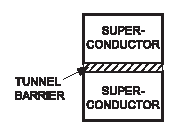
\includegraphics[width=0.25\textwidth]{jj_schematic.pdf}}
	\subfigure[]{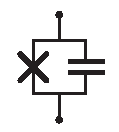
\includegraphics[width=0.18\textwidth]{jj_circuit.pdf}}
	\subfigure[]{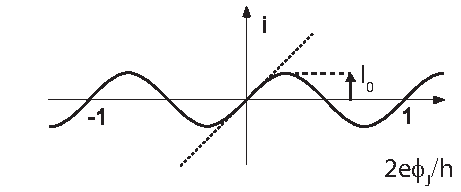
\includegraphics[width=0.5\textwidth]{jj_current.pdf}}
	\caption{Characteristics of the Josephson junction. (a) Physical schematic: insulator layer. (b) Circuit schematic: tunnel in parallel with capacitor. (c) Current-flux relation. Dashed line is relation for linear inductor of equivalent effective inductance. From \cite{vool2017introduction}.}
	\label{fig_jj}
\end{figure}

The circuit behaviour of Josephson junctions can be modelled by a pure non-linear inductor and a capacitor in parallel. The current through and flux across a standard inductive element are linearly related by $I(t) = \frac{1}{L} \phi_L(t)$. In a Josephson junction, this current-flux relation is non-linear by 
\begin{equation}
I(t) = \frac{\phi_0}{L_J} \sin{\left(\frac{\phi(t)}{\phi_0}\right)} = \frac{\phi_0}{L_J} \sin{\varphi_J(t)} 
\end{equation}
The junction is periodic in flux over the superconducting flux quantum $\phi_0 \equiv \frac{\hbar}{2e}$, related to the Cooper pair charge $-2e$. Above we have defined $\varphi = \frac{\phi}{\phi_0}$, the dimensionless `gauge invariant phase'.  Note that an alternate convention is $\phi_0 \equiv \frac{h}{2e}$ and $\varphi = \frac{2\pi}{\phi_0}$ (we will not use this definition). The characteristic current is $I_0 \equiv \frac{\phi_0}{L_J}$. By integration, the energy of the josephson junction energy is
\begin{equation}
E = - \frac{\phi_0^2}{L_J} \cos{\left(\frac{\phi}{\phi_0}\right)} = - E_J \cos{\varphi},
\hspace{1cm}
E_J \equiv \frac{\phi_0^2}{L_J}
\end{equation}
This nonlinearity will prove crucial to producing anharmonic potentials.



\subsection{Setting up the circuit Lagrangian}

We will work with the method of nodes. (Note that the alternative method of loops is equivalent and dual.) Using the dynamic variable $\varphi$, the phase across each element, the energy contributions of pure inductive, capacitative, and junction elements are 
\begin{equation}
E_\text{capacitor} = \frac{1}{2} C \phi_0^2 \dot{\varphi}^2
\hspace{1cm}
E_\text{inductor} = \frac{1}{2} E_L \varphi^2
\hspace{1cm}
E_\text{junction} = - E_J \cos{\varphi}
\label{equ_elementenergies}
\end{equation}
Where $E_L=\frac{\phi_0^2}{L}$. In subsequent discussion it will also be convenient to define $E_C = \frac{e^2}{2C}$. Recall that a Josephson junction should be treated as a pure capacitor and and pure junction in parallel.

To form the Lagrangian, a spanning tree connecting all nodes in the circuit is chosen and each branch of the tree is labelled by a flux (or phase). These branch fluxes are the coordinates and those forming a closed loop (connected by inductors and junctions) must satisfy
\begin{equation}
\sum_\text{around loop} \phi = \phi_\text{ext}
\end{equation}
where $\phi_\text{ext}$, the flux offset, captures the static flux enclosed by the loop formed by the branches. \cite{vool2017introduction}. These constraints reduce the number of branches in the circuit to the true degree of freedom. $\lagr = T - V$ is then constructed additively, where each capacitor contributes to $T$ and each inductor and junction to $V$ according to Equation \ref{equ_elementenergies}. We saw that node charges are conjugate momenta to the node fluxes and the Hamiltonian is constructed by the usual transformation.

It may be more convenient to work instead with node fluxes. Then the coordinates are the flux (or phase) at each node, and the same formulation follows. The node fluxes are related to the branch fluxes simply by $\phi_b = \phi_A - \phi_B$, where the branch $b$ connects the nodes $A$ and $B$.



\subsection{Quantisation}

In the quantum formulation, the flux, charge, and circuit Hamiltonian are operators:
\begin{equation}
\phi \rightarrow \hat{\phi}, \quad
q \rightarrow \hat{q}, \quad
\ham \rightarrow \hat{\ham}
\end{equation}
Because flux and charge are conjugate variables proper, we can note the analogy to the spatial position $\hat{\phi} \longleftrightarrow \hat{x}$ and conjugate momentum $\hat{q} \longleftrightarrow \hat{p}$. Their commutation relationship 
\begin{equation}
\comm{\hat{x}}{\hat{p}} = i \hbar
\end{equation}
motivates
\begin{equation}
\comm{\hat{\phi}}{\hat{q}} = i \hbar
\end{equation}
Recalling $\varphi = \frac{2e}{\hbar} \phi$ and introducing $n = \frac{1}{2e} q$, the quantised charge number, we can make the transformation to dimensionless conjugate operators $\hat{\varphi}$ and $\hat{n}$ related by
\begin{equation}
\comm{\hat{\varphi}}{\hat{n}} = i
\end{equation}
From now, we omit the operator hat notation for brevity. The relationships for position and momentum
\begin{equation}
p = \pdv{\lagr}{\dot{x}}
\hspace{1cm}
p = - i \hbar \pdv{}{x}
\end{equation}
motivates for the conjugate flux and charge variables, or phase and charge number variables
\begin{equation}
q = \pdv{\lagr}{\dot{\phi}}
\hspace{1cm}
q = -i \hbar \pdv{}{\phi}
\end{equation}
\begin{equation}
n = \frac{1}{\hbar} \pdv{\lagr}{\dot{\varphi}}
\hspace{1cm}
n = -i\pdv{}{\varphi}
\end{equation}
The Hamiltonian can than be derived as 
\begin{equation}
\ham = \hbar \sum n \dot{\varphi} - \lagr 
= \sum \pdv{\lagr}{\dot{\varphi}} \dot{\varphi} - \lagr
\end{equation}

The above relationships allow us to transform between the phase and charge number bases. Though we will almost exclusively use the (continuous) phase basis in this paper, the same systems can be described and numerically solved in the (discrete) charge number space. 




\section{Superconducting qubits}



\subsection{Qubit lifetime}

Recent work on superconducting qubits has sought to increase qubit lifetime - the time for which a qubit retains its quantum information. Two standard measures of a qubit's coherence timescale are $T_1$ and $T_2$. \cite{schuster2007circuit}.

The relaxation timescale $T_1$ captures the energy dissipation from the system, which tends to relax to its ground state.
\begin{equation}
\ket{\psi} = \delta \ket{0} + (1-\delta) \ket{1}
\end{equation}
For small $\delta$. Experimentally, $T_1$ can be measured as the decay timescale of the $\ket{1}$ state. A $\pi$ pulse is applied to a $\ket{0}$ initialised qubit and the probability of measuring the $\ket{1}$ state is measured with different waiting times to recover the decay curve (Figure \ref{fig_coherence}a). 

The dephasing timescale $T_2$ captures the loss of phase information from the system. Entanglement with the environment causes unpredictable phase evolution by introducing noise to the eigenenergies.
\begin{equation}
\ket{\psi} = e^{-\frac{(E_0 + \delta E_0)}{\hbar} t} \ket{0} + e^{-\frac{(E_1 + \delta E_1)}{\hbar} t} \ket{1}
\end{equation}
Experimentally, $T_2$ can be measured by observing the decaying envelope of Ramsey fringes. This involves applying two $\pi/2$ pulses separated by waiting time $\Delta T$. The probability of flipping states oscillates with $\Delta T$, modulated by a envelope whose amplitude decays from the $T_2$ (Figure \ref{fig_coherence}b). An alternative method is spin-echo measurement.

\begin{figure}[H]
	\centering
	\subfigure[$T_1$ measurement.]{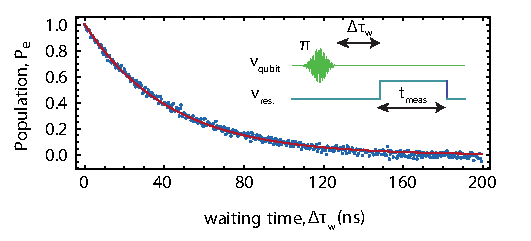
\includegraphics[width=0.44\textwidth]{t1relax.pdf}}
	\subfigure[$T_2$ measurement (Ramsey fringes).]{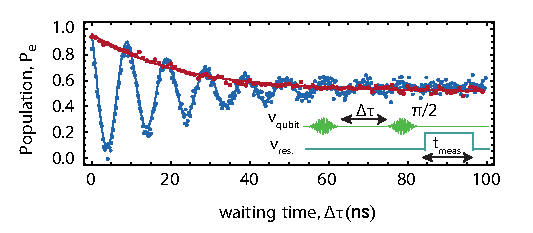
\includegraphics[width=0.48\textwidth]{t2ramsey.pdf}}
	\caption{Measurement of coherence times for an example qubit. From \cite{scarlino2017all}.}
	\label{fig_coherence}
\end{figure}

In general, $T_1 > T_2$, and typically $T_1 >> T_2$. We will see how certain qubit properties lead to long-lived qubits with large $T_1$ and $T_2$.




\subsection{Cooper pair box}

\begin{figure}[H]
	\centering
	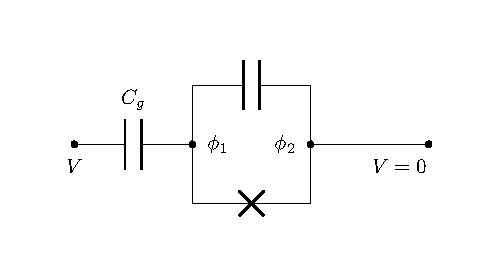
\includegraphics[trim={0cm 1cm 0cm 1cm}, clip, width=0.5\textwidth]{cpb.pdf}
	\caption{Cooper pair box qubit with junction energy $E_J$ and capacitance $C$ (an effective capacitance capturing the lumped capacitance from the junction and pure capacitor). It is capacitatively coupled (for qubit control) via a capacitor of magnitude $C_g$ to the external voltage bias $V$.}
	\label{fig_cpb}
\end{figure}

The Cooper pair box is the simplest superconducting qubit, comprising a Josephson junction and capacitor in parallel. \cite{girvin2011superconducting}. Figure \ref{fig_cpb} shows the qubit in its most straightforward coupling configuration. With $\phi_1, \phi_2$ as labelled, the Lagrangian is
\begin{align}
\lagr 
&= \frac{1}{2} C_g (\dot{\phi}_1 - V)^2 + \frac{1}{2} C (\dot{\phi}_1 - \dot{\phi}_2)^2 + E_J \cos{\left(\frac{\phi_1 - \phi_2}{\phi_0}\right)} \\
&= \frac{1}{2} C_g \phi_0^2 \left(\dot{\varphi}_1 - \mathcal{V}\right)^2 + \frac{1}{2} C \phi_0^2 (\dot{\varphi}_1 - \dot{\varphi}_2)^2 + E_J \cos{(\varphi_1 - \varphi_2)}
\end{align}
where $\mathcal{V} = V / \phi_0$. We identify by inspection a \emph{compact} variable $\varphi_1-\varphi_2$, that is, a variable whose values are bounded because the Lagrangian depends on it periodically. (Note that a compact variable is conjugate with a discrete variable, which for superconducting qubits is the quantised charge on a charge island.) In particular, $\varphi_1-\varphi_2$ and $\varphi_1-\varphi_2+2\pi k, \ k \in \mathbb{Z}$ are physically indistinguishable, and this translational invariance must be respected in the numerical analysis. This motivates the basis transformation
\begin{equation}
\theta = \frac{1}{2} (\varphi_1 - \varphi_2)
\hspace{1cm}
\Sigma = \frac{1}{2} (\varphi_1 + \varphi_2)
\end{equation}
where $\theta$ is compact, and $\Sigma$ is the sum of the phases, which must be a constant of motion (`centre of mass' movement). $\theta$ and $\Sigma$ are orthogonal. Substitution gives
\begin{align}
\lagr 
&= \frac{1}{2} C_g \phi_0^2 \left((\dot{\theta} + \dot{\Sigma}) - \mathcal{V}\right)^2 + \frac{1}{2} C \phi_0^2 \dot{\theta}^2 + E_J \cos{\theta}
\end{align}
Because the potential is $\Sigma$-independent, it is indeed a constant of motion and we can transform to the reference frame where $\dot{\Sigma}=0$. Also dropping constant terms ($\mathcal{V}^2$ in the expansion of the first term), the Lagrangian simplifies to
\begin{equation}
\lagr = \frac{1}{2} \phi_0^2 (C + C_g) \dot{\theta}^2 - C_g \phi_0 V \dot{\theta} + E_J \cos{\theta}
\end{equation}
The conjugate charge number is
\begin{equation}
n 
= \frac{1}{\hbar} \pdv{\lagr}{\dot{\theta}}
= \frac{1}{\hbar} \phi_0^2 (C + C_g) \dot{\theta} - \frac{1}{\hbar} \phi_0 C_g V
\implies
\dot{\theta} = \frac{\hbar n + \phi_0 C_g V}{\phi_0^2 (C + C_g)}
\end{equation}
Thus the Hamiltonian $\ham = \hbar n \dot{\theta} - \lagr$ is given by
\begin{align}
\ham 
&= \frac{1}{2} \phi_0^2 (C + C_g) \frac{\left(\hbar n + \phi_0 C_g V\right)^2}{\phi_0^4 (C + C_g)^2} - E_J \cos{\theta} \\
&= \frac{(2e)^2}{2 (C + C_g)} \left(n + \frac{\phi_0}{\hbar} C_g V\right)^2 - E_J \cos{\theta} \\
&= 4 E_C (n - n_g)^2 - E_J \cos{\theta}
\end{align}
where $E_C = \frac{e^2}{2 (C + C_g)}$ and the gate charge $n_g = - \frac{C_g V}{2e}$. 

This is the standard form of the Cooper pair box Hamiltonian. It is straightforward to express it in purely in the phase basis by ($n=-i\partial_\theta$), where the eigenvalue problem $H \ket{\psi} = E \ket{\psi}$ takes the form of the Matthieu equation with Matthieu functions as the solutions. \cite{girvin2011superconducting}. In the charge number basis,
\begin{equation}
\ham = \sum_n \left(4 E_C (n - n_g)^2 \ket{n} \bra{n} - \frac{E_J}{2} (\ket{n} \bra{n+1} + \ket{n+1} \bra{n})\right),
\end{equation}
and it is straightforward to identify the eigenstates as the set $\ket{n}$ representing the number of Cooper pairs tunneled through the Josephson junction.




\subsection{Transmon}

\begin{figure}[H]
	\centering
	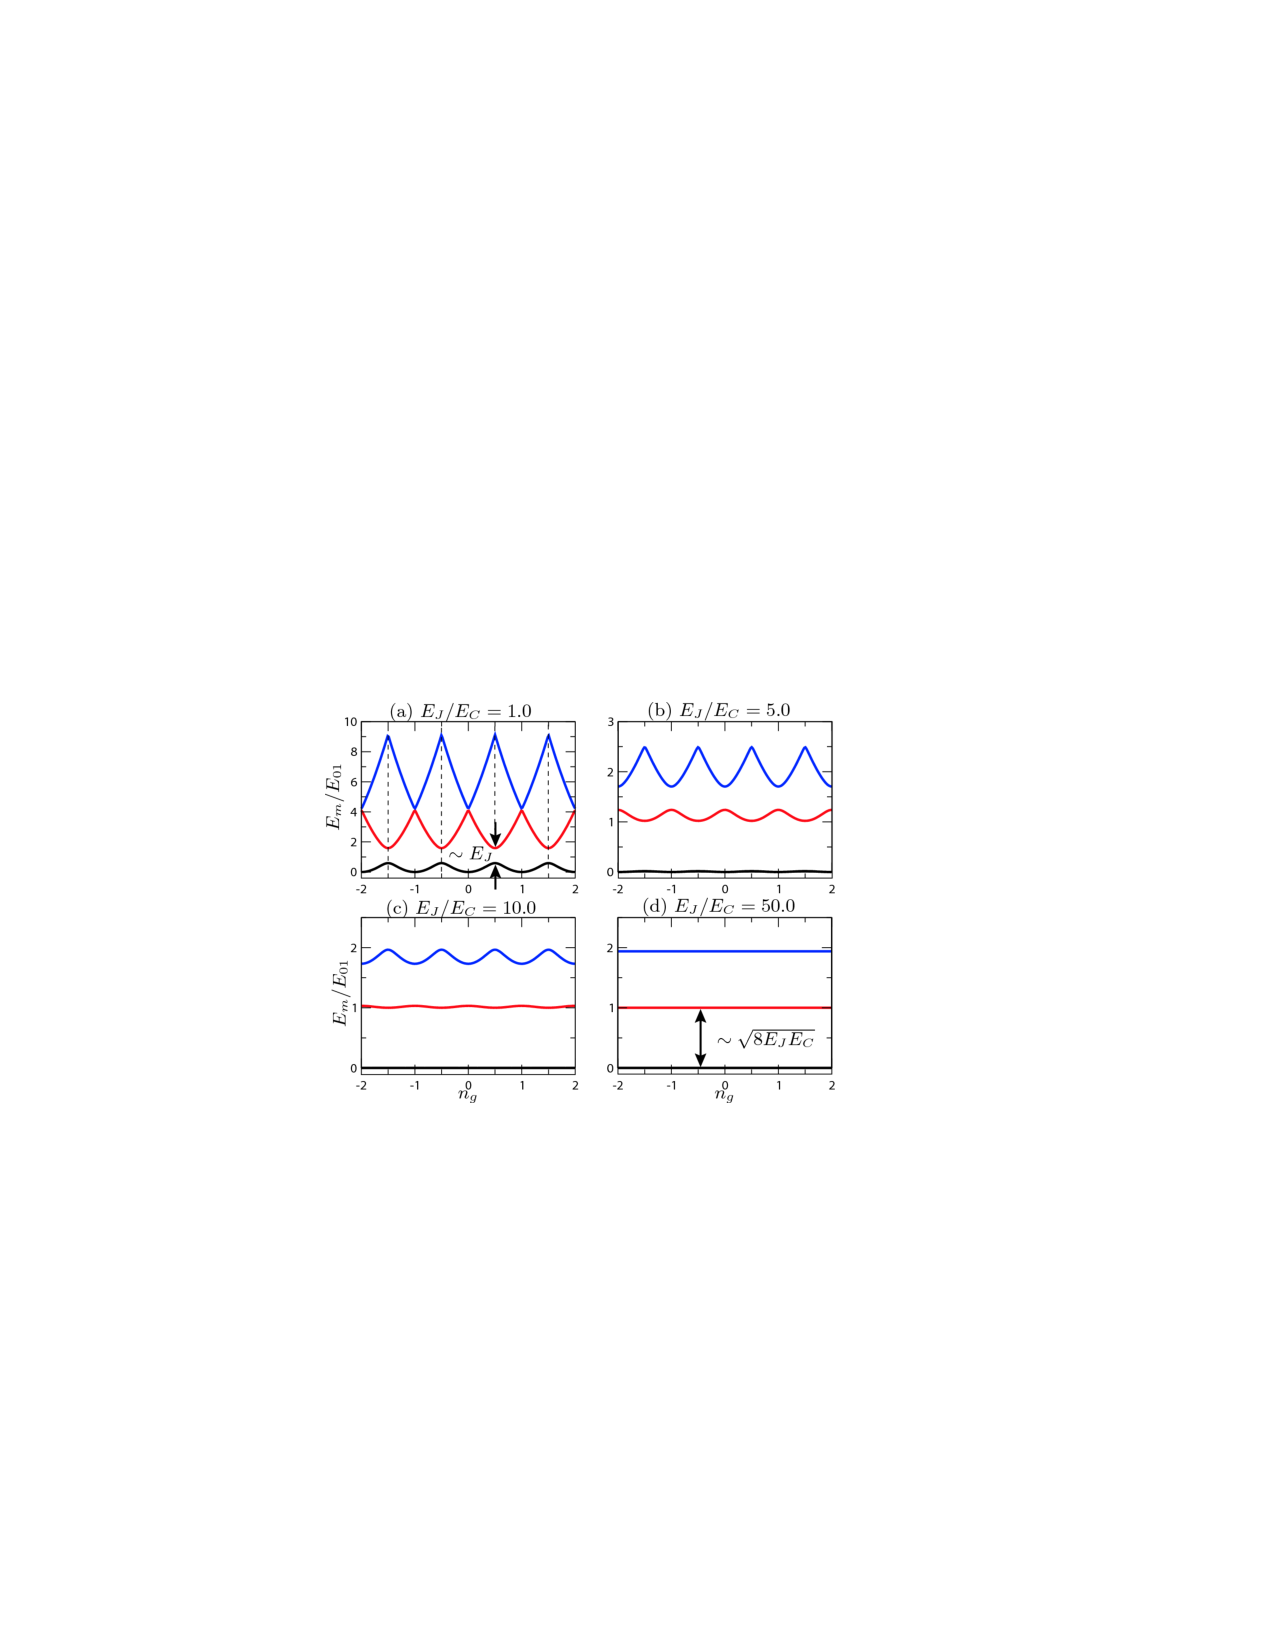
\includegraphics[width=0.5\textwidth]{cpb_energies.pdf}
	\caption{First three eigenenergies of the Cooper pair box as a function of $n_g$. Energies are in units of transition energy $E_{01}$ evaluated at $n_g=1/2$. From \cite{koch2007charge}.}
	\label{fig_cpbenergies}
\end{figure}

The Cooper pair box is highly susceptible to dephasing due to its eigenenergies' dependence on gate charge $n_g$. Though several `sweet spots' of first-order insensitivity to $n_g$ exist at half integer $n_g$, global insensitivity is achieved in the transmon regime (Figure \ref{fig_cpbenergies}). The transmon is a Cooper pair box with $E_J/E_C >> 1$. \cite{koch2007charge}.

In a transmon, the large capacitance screens the junction from $n_g$ fluctations, resulting charge noise insensitivity of the energy spectrum. This robustness preserves the transition frequency between the transmon's ground and first excited states and increases $T_2$.

However, in this same limit, the transmon approaches the LC-oscillator and suffers from anharmonicity. Figure \ref{fig_cpbenergies} shows the increased similarity in level spacings as $E_J/E_C$ increases. This is undesirable as microwave pulses intended to cause transitions between $\ket{0}$ and $\ket{1}$ could cause leakage to higher excited states. A second fundamental limitation is the transmon's lack of disjointness. Because its potential is a single cosine well, its eigenstates are simlarly localised and couple easily. The ease of unintended state transitions makes the transmon highly susceptible to ground state relaxation to the detriment of $T_1$.




\subsection{Fluxonium}

The fluxonium qubit comprises a Josephson junction, whose capacitative and junction components have comparable energies ($E_C \approx E_J$), in parallel with a large linear inductor ($E_L << E_J$). \cite{earnest2018realization}.

\begin{figure}[H]
	\centering
	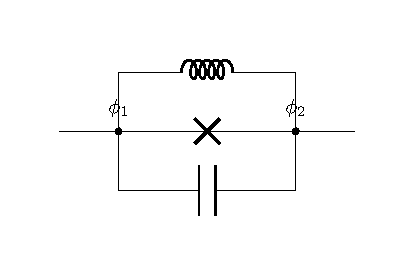
\includegraphics[trim={0cm 1cm 0cm 1cm}, clip, width=0.5\textwidth]{fluxonium.pdf}
	\caption{Fluxonium with junction energy $E_J$, charging energy $E_C$, and inductive energy $E_L$.}
	\label{fig_fluxonium}
\end{figure}

In the following analysis we will consider the uncoupled fluxonium in isolation. We must account for $\varphi_\text{ext} = \phi_\text{ext} / \phi_0$ in the closed loop (containing the junction and linear inductor) and choose to work in the branch flux, $\phi=\phi_2-\phi_1, \ \varphi=\phi/\phi_0$. The Lagrangian is
\begin{equation}
\lagr = \frac{1}{2} E_L \varphi^2 + E_J \cos{\left(\varphi - \varphi_\text{ext}\right)} - \frac{1}{2} C \phi_0^2 \dot{\varphi}^2
\end{equation}
with the conjugate charge number $n = -i \partial_\varphi$. Thus the Hamiltonian is
\begin{equation}
\ham = - 4 E_C \partial_\varphi^2  - E_J \cos{\left(\varphi - \frac{\phi_E}{\phi_0}\right)} + \frac{1}{2} E_L \varphi^2
\end{equation}
The fluxonium energy landscape depends on the external flux through the closed loop. Ideally, circuit parameters and $\phi_\text{ext}$ are such that the lowest energy eigenstates are disjoint \emph{fluxons} localised in separate wells as opposed to \emph{plasmons} localised in the same well, and so $\matrixel{0}{n}{1} \approx 0$ (Figure \ref{fig_fluxoniumenergies}b). As tunneling is exponentially suppressed ($\propto \exp(-E_J/E_C)$) by the barrier separating the wells, there is low probability of leakage between $\ket{0}$ and $\ket{1}$, increasing $T_1$. 

Due to this same disjointness, qubit control requires a multistep Raman transition using an excited plasmon level (with nonzero coupling matrix element with both $\ket{0}$ and $\ket{1}$) as the intermediate state. It is unlikely for this complex transition to take place due to noise.

\begin{figure}[H]
	\centering
	\subfigure[$\varphi=0.02(2\pi)$.]{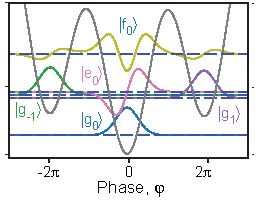
\includegraphics[width=0.35\textwidth]{fluxoniumenergies1.pdf}}
	\subfigure[$\varphi=0.51(2\pi)$. Potential resembles symmetric double well with near degenerate $\ket{g_0}$ and $\ket{g_1}$.]{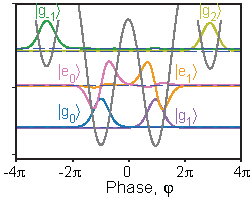
\includegraphics[width=0.34\textwidth]{fluxoniumenergies2.pdf}}
	\caption{Potential landscape, eigenenergies, and eigenstates for the fluxonium for two different $\phi_\text{ext}$. From \cite{earnest2018realization}.}
	\label{fig_fluxoniumenergies}
\end{figure}

The primary disadvantage of the fluxonium is its high sensitivity to external flux. Noisy fluctuations shift the entire energy landscape, causing $T_2$ dephasing (and $T_1$ relaxation due to unexpected level transitions if changes do not take place adiabatically). Moreover, the advantageous disjointness property is only achieved at some external flux values. For example, for small $\varphi_\text{ext}$ (and large $E_C$), the lower level eigenstates are plasmons co-localised in a single potential well and the fluxonium behaves lke a transmon. Unfortunately, this possibly noisy external parameter is critical to good fluxonium design.




\subsection{Transitions and qubit control}

In real atoms, energy eigenstate transitions can be driven by coupling with electric field. The interacting Hamiltonian term is given by
\begin{equation}
H_\text{coupling} = - \vec{E} \cdot \vec{p}
\end{equation}
where $\vec{E}$ is the field and $\vec{p}$ is the dipole moment of the atom. Results from time dependent perturbation theory show that for a perturbing term of sinusoidal time dependence, $\tilde{H}(\vec{r}, t) = U(\vec{r}) \cos{\omega t}$, the probability that a state initialised to $\ket{i}$ is found in state $\ket{j}$ at time $t$ is
\begin{equation}
P_{i \rightarrow j} \approx \frac{\abs{U_{ij}}^2}{\hbar^2} \frac{\sin^2{(\omega_0-\omega)t/2}}{(\omega_0-\omega)^2}
\end{equation}
where $\omega_0=(E_j - E_i)/\hbar$ is the transition frequency. Thus the transition rate depends on the coupling off-diagonal matrix element of the perturbing potential in the eigenbasis, and the discrepancy between the driving and transition frequencies. It is maximised at $\omega_0=\omega$, consistent with Fermi's golden rule.

From cavity QED, an analogous dipole moment can be derived for the artificial atom that is the qubit. Because superconducting qubits are of micrometre order and have microwave excitation frequencies (wavelength $\sim \SI{e-2}{\metre}$), the oscillatory $E$ field can be approximated as constant across the device. Thus $\matrixel{i}{d_\text{qubit}}{j}$ characterises the coupling strength, where the qubit dipole $d_\text{qubit}$ depends on both the circuit design and coupling configuration. 
\begin{comment}
Also in analogy with electron dipole selection rules for the atom, transitions are restricted (must be between states of different parity).
\end{comment}

Physically, the qubit is capacitatively coupled to an electric field by placing it in a resonant cavity. (Cavity measurements also constitute the non-demolition qubit readout.) For example, for the transmon with capacitance $C$, coupled by a capacitance $C_C$,
\begin{equation}
H_\text{coupling} = 2e \frac{C_C}{C + C_C} \hat{V} \otimes \hat{n} 
\end{equation}
which is the cross-term that interacts $V$ and $n$ in the Cooper pair box Hamiltonian. The result that $H_\text{coupling} \propto \hat{V} \otimes \hat{n}$ holds generally. These two operators are quantised as 
\begin{equation}
\hat{V} = V_{rms} (\hat{a} + \hat{a}^\dagger),
\quad
V_{rms} = \sqrt{\frac{\hbar \omega_R}{2 C_R}}
\hspace{2cm}
\hat{n} = \sum_{i,j} \matrixel{i}{\hat{n}}{j} \ket{i} \bra{j} = \frac{1}{\hbar} \pdv{\varphi}
\end{equation}
where the cavity is modelled as a harmonic LC oscillator with effective parameters $L_R, C_R$ and natural frequency $\omega_R = \frac{1}{\sqrt{L_R C_R}}$.  $V$ acts on the space of photons with the creation and annihilation operators and $n$ on the qubit states with the charge number operator (alternatively, $\hat{n} = \frac{1}{\hbar} \pdv{\varphi}$ in the phase basis). 

This quantisation for $V$ is motivated in \cite{girvin2011superconducting} from the LC harmonic oscillator. Briefly, its Hamiltonian
\begin{equation}
\ham = \frac{\phi^2}{2L_R} + \frac{q^2}{2C_R} = \hbar \omega_R \left(\hat{a}^\dagger \hat{a} + \frac{1}{2}\right)
\end{equation}
suggests that
\begin{equation}
\hat{a} = + i \frac{1}{\sqrt{2 \hbar L_R \omega_R}} \hat{\phi} + \frac{1}{\sqrt{2 \hbar C_R \omega_R}} \hat{q}
\hspace{1cm}
\hat{a}^\dagger = - i \frac{1}{\sqrt{2 \hbar L_R \omega_R}} \hat{\phi} + \frac{1}{\sqrt{2 \hbar C_R \omega_R}} \hat{q}
\end{equation}
Substituting for $\hat{q}$ in terms of the creation and annihilation operators into the definition of $\phi$ as the time integral of potential
\begin{equation}
\hat{V} = \dv{\hat{\phi}}{t} = \frac{i}{\hbar} \comm{\ham}{\hat{\phi}} = \frac{1}{C_R} \hat{q}
\end{equation}
gives the expression for $\hat{V}$.

\begin{comment}
[More content on cavity coupling and non demolition readout of qubit state?]
\end{comment}




\subsection{Design objectives}

From the theory presented above emerge several desirable properties of qubits.

\textbf{Nondegeneracy.} It is difficult to selectively make transitions to degenerate eigenstates excited by photons of the same frequency. Even near-degeneracies are problematic: suppose eigenstates $\psi$ and $\psi'$ are near-degenerate with separation $\delta E$. Pulses that drive a transition to $\psi$ but minimally drive $\psi'$ must be sharply peaked in frequency space, with characteristic width upper bounded by $\sim \delta \omega = \delta E / \hbar$. In the time domain, this pulse has characteristic width $\tau \propto 1 / \delta E$ (energy and time being complementary Fourier variables). This sets a fundamental limit on the speed per bitwise operation.

\textbf{Anharmonicity.} As a generalisation of the nondegeneracy condition, evenly spaced eigenergies in a harmonic potential impede fast, accurate control. For a harmonic oscillator (such as the LC circuit), the same frequency drives transitions between states of interest and between arbitrary states: the driving frequency for $\ket{0}$-$\ket{1}$ also drive $\ket{1}$ to $\ket{2}$, $\ket{2}$ to $\ket{3}$, etc, resulting in leakage to higher energy levels. Near-harmonic energies are similarly problematic and limit gate speed.

\textbf{Insensitivity to external parameters} such as gate charge and external flux, which are difficult to control experimentally, makes a qubit robust against noise. In particular, if level spacings $E_i-E_j$ are insensitive to environmental parameters, dephasing is minimised and $T_2$ is improved. Moreover, fast, non-adiabatic fluctuations might not preserve eigenstate populations, so this robustness also improves $T_1$.

\textbf{Disjoint support}. Quantum information is corrupted when the environment and qubit couple to cause unexpected state transitions. We saw that for a perturbative $\tilde{H}$,
\begin{equation}
P(\text{transition between states } i, j) \propto |\matrixel{i}{\tilde{H}}{j}|^2.
\end{equation}
If $\ket{i}, \ket{j}$ are disjoint (not similarly localised), this matrix element is $\approx 0$ and the effective dipole moment for this transition is `suppressed'. Thus noise is unlikely to cause $\ket{i}$-$\ket{j}$ transitions, provided there is no path of non-disjoint intermediate states between $\ket{i}$ and $\ket{j}$. This generally produces longer $T_1$.

\begin{comment}
[The matrix element can be 0 for symmetry reasons between $\psi_1$ and $\tilde{H} \psi_2$ even when they're co-localised, e.g. odd and even functions. However, this is generally less robust to noise.]
\end{comment}

The disjointness condition evokes the struggle between conflicting objectives of weak coupling to minimise noisy transitions and strong coupling for easy control. To transition between disjoint $\ket{0}$ and $\ket{1}$ states, \textbf{an intermediate transition level} which couples to both $\ket{0}$ and $\ket{1}$, but is more energetic than both $\ket{0}$ and $\ket{1}$ can be used in a multistep driving process that is unlikely to be caused by noisy fluctuations.

We present some intuition for identifying parameters that promote the above objectives. Generally, the system potential is described by a harmonic well with steepness $E_L$, due to the linear inductance, perturbed by sinusoidal oscillations of magnitude $E_J$, due to the junction term. If $E_J$ is large relative to $E_L$, the potential is multiwell and accessible from the ground state are both intra-well plasmons (e.g. $\ket{g_0} \leftrightarrow \ket{e_0}$ in Figure \ref{fig_fluxoniumenergies}) and disjoint inter-well fluxons (e.g. $\ket{g_0} \leftrightarrow \ket{g_1}$ in Figure \ref{fig_fluxoniumenergies}). The capacitative term is kinetic and $E_C$ is inversely related to the system's effective mass. Increasing $E_C$ increases level spacings, the probability of inter-well tunelling, and hybydisation between fluxon states.




\section{Trifluxonium}

\subsection{Circuit Hamiltonian}

\begin{figure}[H]
	\centering
	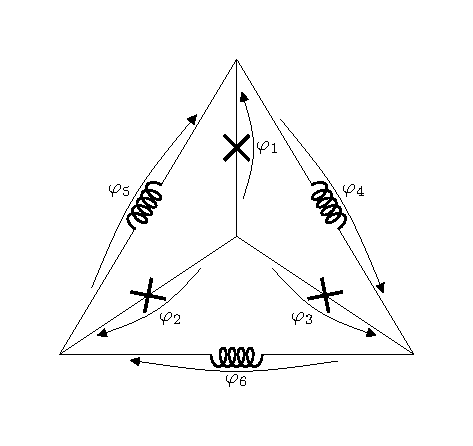
\includegraphics[trim={0cm 1cm 0cm 1cm}, clip, width=0.4\textwidth]{triflux_branch.pdf}
	\caption{Trifluxonium. Each inductor is parametrised by inductive energy $E_L$ and each Josephson junction by inductive energy $E_J$ and capacitative energy $E_C$.}
	\label{fig_triflux}
\end{figure}

The isolated (uncoupled) trifluxonium qubit is presented in Figure \ref{fig_triflux}. We work with branch phases $\{\varphi_i\}, \ i=1,...,6$ as labelled. The kinetic and potential energies of the system are
\begin{align}
T &= \frac{1}{2} C_J \phi_0^2 (\dot{\varphi_1}^2 + \dot{\varphi_2}^2 + \dot{\varphi_3}^2) \\
V &= -E_J (\cos{\varphi_1} + \cos{\varphi_2} + \cos{\varphi_3}) + \frac{1}{2} E_L (\varphi_4^2 + \varphi_5^2 + \varphi_6^2)
\end{align}
As a first order approximation, assume the same external flux $\phi_E=\phi_0 \varphi_E$ is enclosed by each of the three loops. 
\begin{equation}
\varphi_1 + \varphi_4 - \varphi_3 = \varphi_E
\hspace{1cm}
\varphi_3 + \varphi_6 - \varphi_2 = \varphi_E
\hspace{1cm}
\varphi_2 + \varphi_5 - \varphi_1 = \varphi_E
\end{equation}
Enforcing the above constraints reduces the system to three degrees of freedom. Further, we make the change of coordinates
\begin{equation}
\zeta = \frac{1}{\sqrt{3}} (\varphi_1 + \varphi_2 + \varphi_3)
\hspace{1cm}
\theta = \frac{1}{\sqrt{2}} (-\varphi_1 + \varphi_3)
\hspace{1cm}
\chi = \frac{1}{\sqrt{6}} (-\varphi_1 + 2 \varphi_2 - \varphi_3)
\end{equation}
This basis change is motivated in the Appendix. In this basis,
\begin{align}
T &= \frac{1}{2} C_J \phi_0^2 (\dot{\zeta}^2 + \dot{\theta}^2 + \dot{\chi}^2) \\
V &= -E_J \left( \cos{\left(\frac{\zeta + \sqrt{2} \chi}{\sqrt{3}}\right)} + 2 \cos{\left(\frac{\theta}{\sqrt{2}}\right)} \cos{\left(\frac{\zeta}{\sqrt{3}} - \frac{\chi}{\sqrt{6}}\right)} \right) + \frac{3}{2} E_L (\theta^2 + \chi^2 + \varphi_E)
\end{align}
As expected, there is one compact variable $\zeta$, conjugate to the quantised variable for the single charge island at the centre of the trifluxonium. The external flux, appearing as an additive constant, has decoupled from the potential and can be dropped. Thus, assuming equal fluxes through the three loops, the trifluxonium is insensitive to external flux.

The Lagrangian is $\lagr = T - V$ and the three conjugate momenta are
\begin{align}
n_\zeta 
= \frac{1}{\hbar} \pdv{\lagr}{\dot{\zeta}} = C_J \phi_0^2 \dot{\zeta}
&\implies \dot{\zeta} = \frac{\hbar}{\phi_0^2 C_J} n_\zeta \\
n_\theta
= \frac{1}{\hbar} \pdv{\lagr}{\dot{\theta}} = C_J \phi_0^2 \dot{\theta}
&\implies \dot{\theta} = \frac{\hbar}{\phi_0^2 C_J} n_\theta \\
n_\chi
= \frac{1}{\hbar} \pdv{\lagr{\dot{\chi}}} = C_J \phi_0^2 \dot{\chi}
&\implies \dot{\chi} = \frac{\hbar}{\phi_0^2 C_J} n_\chi
\end{align}

Thus the Hamiltonian is given by
\begin{equation}
\ham 
= \hbar \left(n_\zeta \dot{\zeta} + n_\theta \dot{\theta} + n_\chi \dot{\chi} \right) - \lagr 
= \frac{1}{2} \hbar^2 \left(\frac{2e}{\hbar}\right)^2 \frac{1}{C_J} (n_\zeta^2 + n_\theta^2 + n_\chi^2) + V
= 4 E_C (n_\zeta^2 + n_\theta^2 + n_\chi^2) + V
\end{equation}
where $E_C = \frac{e^2}{2C}$. Expressing all operators in phase space by the relation $n = -i\pdv{}{\varphi}$, where $n$ is the momentum conjugate to $\varphi$,
\begin{equation}
\ham = -4 E_C \left( \partial_\zeta^2 + \partial_\theta^2 + \partial_\chi^2 \right) - E_J \left( \cos{\left(\frac{\zeta + \sqrt{2} \chi}{\sqrt{3}}\right)} + 2 \cos{\left(\frac{\theta}{\sqrt{2}}\right)} \cos{\left(\frac{\zeta}{\sqrt{3}} - \frac{\chi}{\sqrt{6}}\right)} \right) + \frac{3}{2} E_L (\theta^2 + \chi^2 + \varphi_E)
\end{equation}

Some intuition for the system eigenstates can be gained by visualising the potential (Figure \ref{triflux_potential}). $\theta$ and $\chi$ have quadratic inductive potential terms while $\zeta$ is compact. Thus, the potential sliced along $\zeta$ is a parabolic well and along $\chi$ and $\theta$ parabolic `cylinders', perturbed by cosine fluctuations from the junction terms. Like the one-dimensional fluxonium, the three-dimensional trifluxonium has well structures embedded a large-scale parabolic potentials and can thus accommodate fluxon states. 

\begin{figure}[H]
	\centering
	\subfigure[Constant $\chi$ slice.]{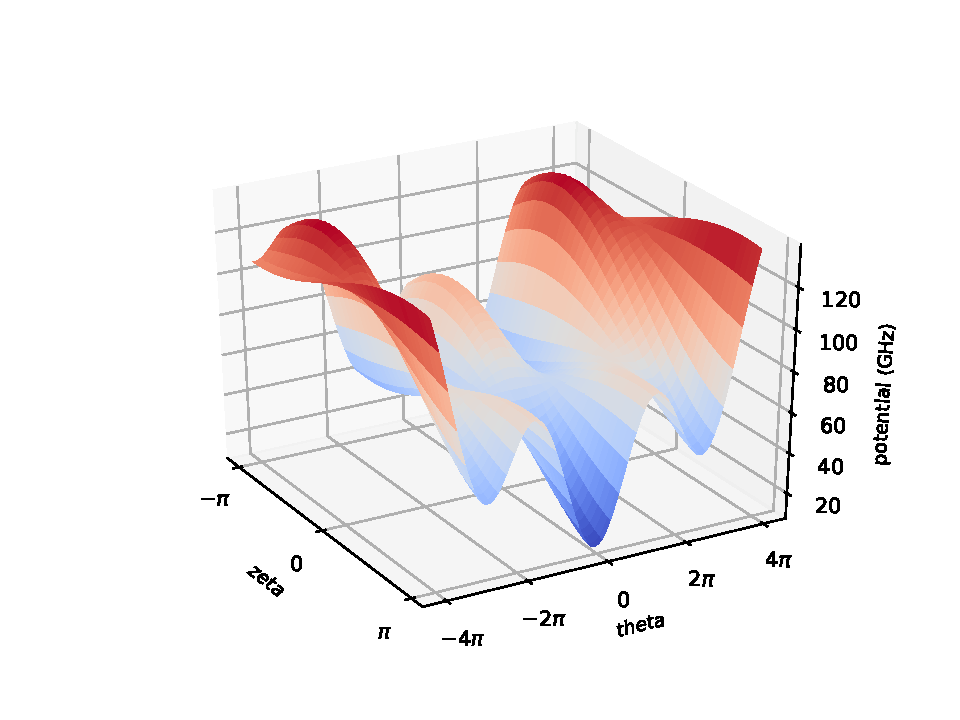
\includegraphics[trim={3cm 1cm 1cm 2cm}, clip, width=0.3\textwidth]{V_zetatheta.pdf}}
	\subfigure[Constant $\theta$ slice.]{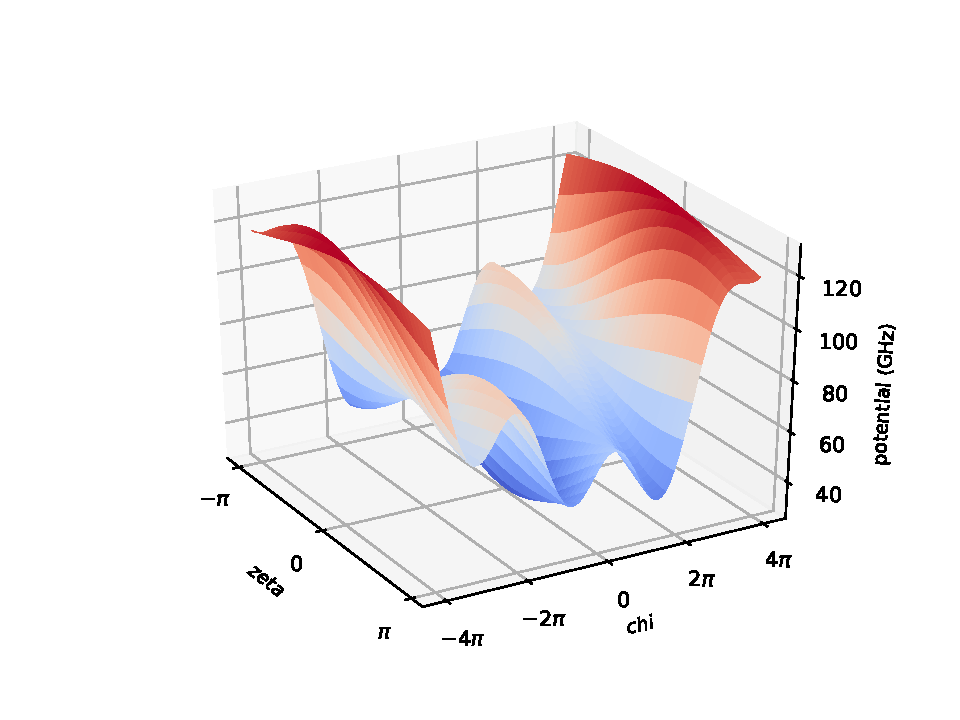
\includegraphics[trim={3cm 1cm 1cm 2cm}, clip, width=0.3\textwidth]{V_zetachi.pdf}}
	\subfigure[Constant $\zeta$ slice.]{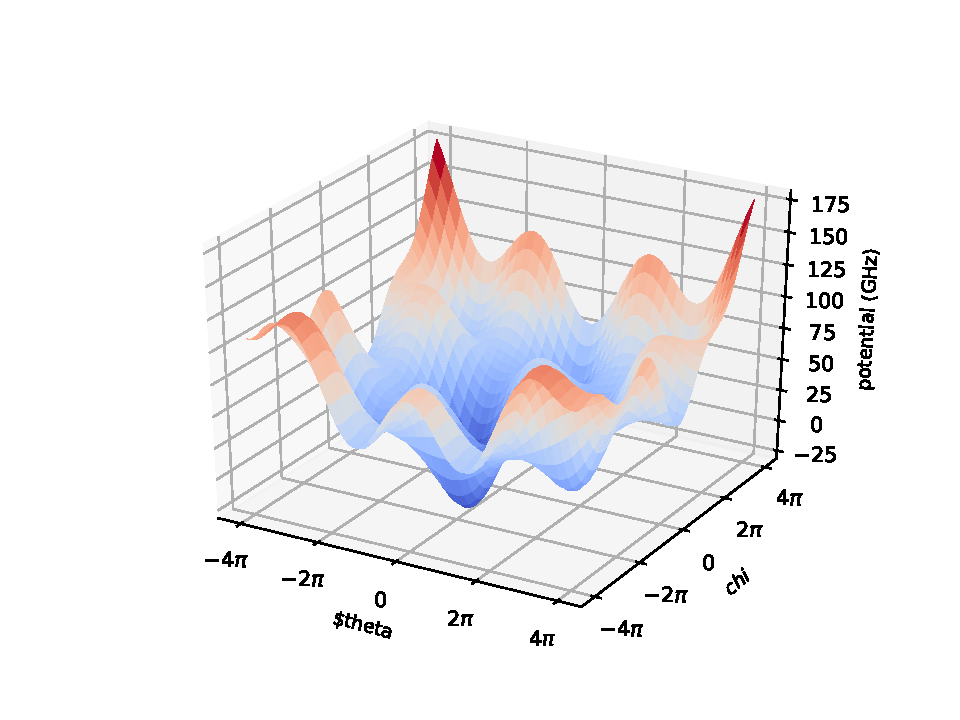
\includegraphics[trim={3cm 1cm 1cm 2cm}, clip, width=0.3\textwidth]{V_thetachi.pdf}}
	\caption{Visualisation of the the three-dimensional trifluxonium potential in two dimensions by examining an arbitrary slice near the centre of the grid along each of the degrees of freedom $\zeta, \theta, \chi$. Parameters $E_C=2, E_J=15, E_L=0.3$, in $\SI{}{\giga\hertz}$ with $h=1$.}
	\label{triflux_potential}
\end{figure}

Further work should consider the qubit's flux dependence when $\phi_\text{ext}$ does vary between the three loops, as would be more realistic in a spatially inhomogeneous magnetic field.



\subsection{Eigensystem}

The Hamiltonian, expressed as a matrix using the finite differences method (refer to Appendix for details), is numerically diagonalised to obtain the system eigenenergies and corresponding eigenstates (eigenvalues and eigenvectors of the discretised Hamiltonian). All energies are in $\SI{}{\giga\hertz}$, in units of $h=1$.

A parameter search over the ballpark experimentally viable values for $E_C, E_J, E_L$ informed the choice of $E_C = \SI{2}{\giga\hertz}, E_J = \SI{15}{\giga\hertz}, E_L = \SI{0.3}{\giga\hertz}$ as `optimal' for the trifluxonium. For this parameter set, Table \ref{tab_eigenenergies} shows the system eigenergies and Figure \ref{fig_estates} shows comprehensively the first ten eigenstates in two-dimensional slices. 

The trifluxonium with these parameters exhibits some desirable qubit properties, which will be discussed below. However, a fundamental limitation of the trifluxonium is due to its strong three-way symmetry (apparent from its circuit diagram), which results in degeneracies. In particular, it is not possible to simultaneously achieve the objectives of anharmonicity and disjoint support, because only by somewhat hybrdising eigenstates through dialling $E_C$ (increasing the kinetic energy relative to `tunnel' height as determined by $E_L$) can the degeneracies be broken, at the cost of losing disjointness. 

Furthermore, disjointness between low-energy states is achieved by bringing the fluxons to a lower energy than the plasmons. As a corollary, the eigenenergies are high, pushing the upper limit of typical transition energies $\sim \SI{10}{\giga\hertz}$. These large single-step transitions are difficult to realise experimentally because they require large power sources, which also dissipate more.

\begin{table}[H]
	\centering
	\begin{tabular}{l l l}
		\hline
		Ground 		& Fluxons 			& Plasmons \\
		\hline
		$E_0 = 0$ 	& $E_1 = 10.88$		& $E_7 = 13.164$ \\
					& $E_2 = 10.881$ 	& $E_8 = 13.618$ \\
					& $E_3 = 10.9$		& $E_9 = 13.619$ \\
					& $E_4 = 10.954$ 	& \\
					& $E_5 = 10.954$ 	& \\
					& $E_6 = 10.97$		& \\
		\hline
	\end{tabular}
	\caption{Numerically simulated lowest ten eigenenergies for the trifluxonium with $E_C = \SI{2}{\giga\hertz}, E_J = \SI{15}{\giga\hertz}, E_L = \SI{0.3}{\giga\hertz}$, grouped into the fluxon and plasmon states. The ground is normalised to energy 0. All energies in $\SI{}{\giga\hertz}$.}
	\label{tab_eigenenergies}
\end{table}

\begin{figure}
	\centering
	\subfigure[Constant $\chi$ slice.]{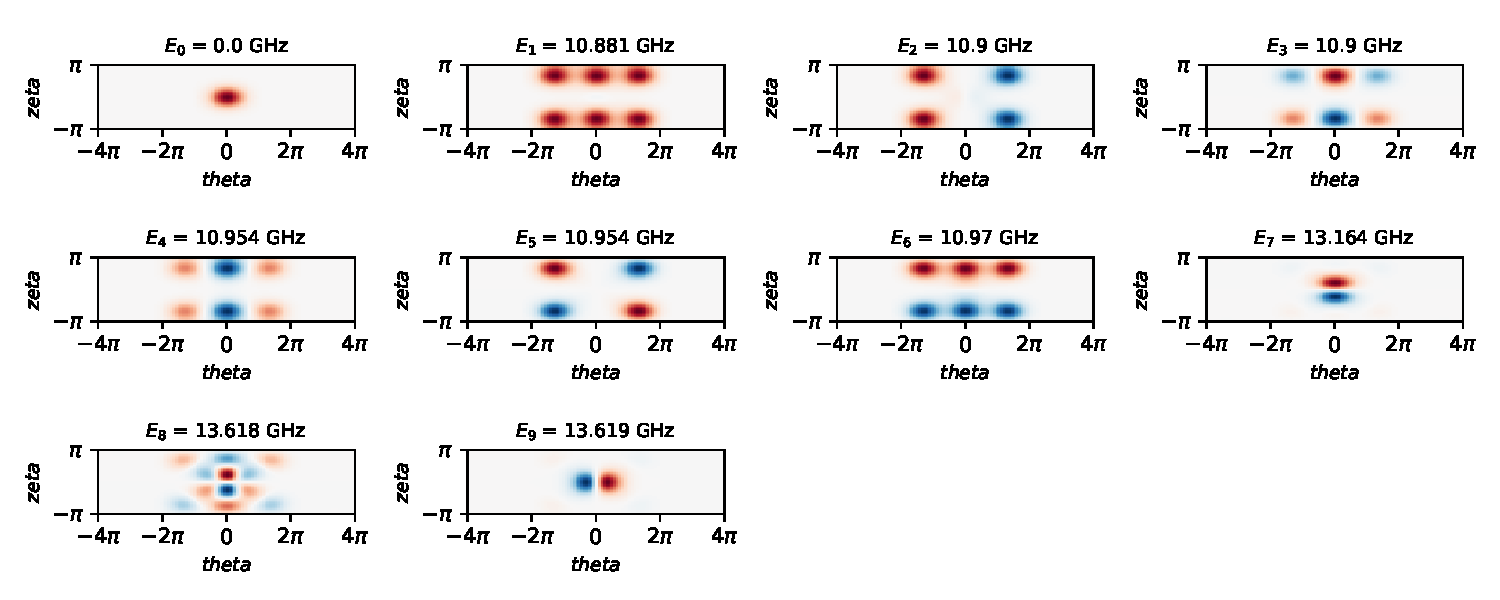
\includegraphics[trim={0cm 0.3cm 0cm 0cm}, clip, width=0.9\textwidth]{zetatheta.pdf}}
	\subfigure[Constant $\theta$ slice.]{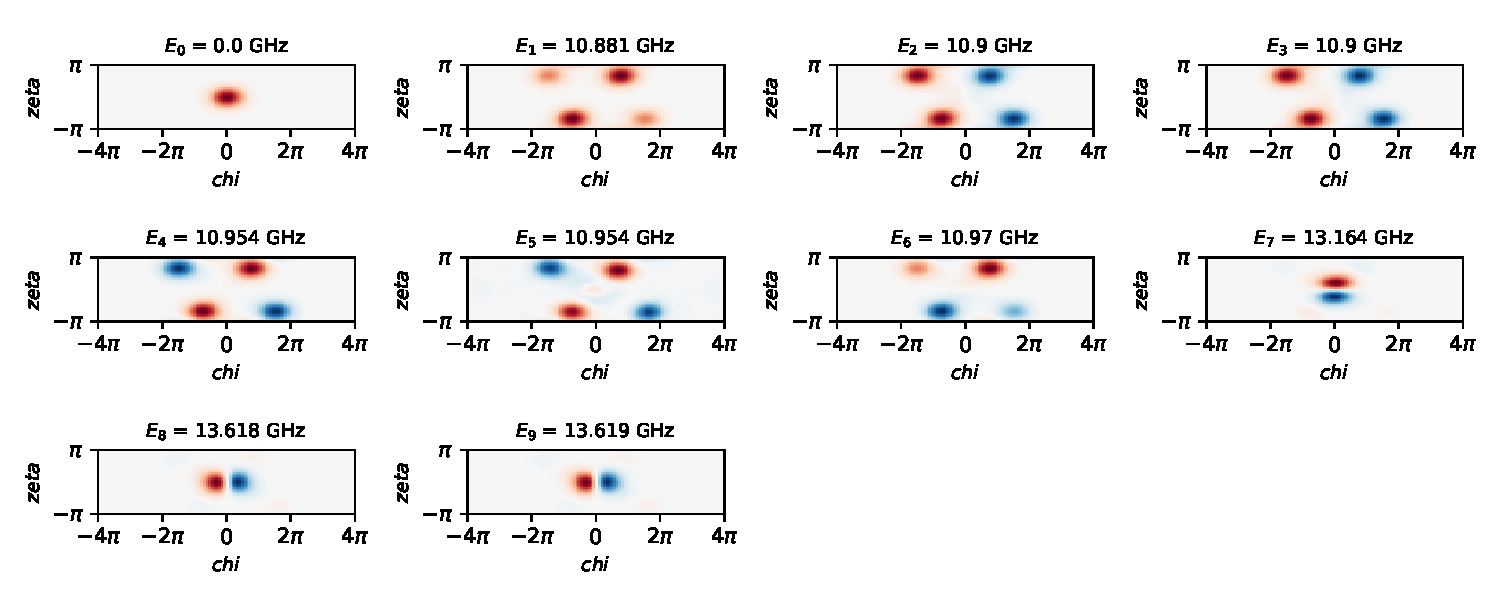
\includegraphics[trim={0cm 0.3cm 0cm 0cm}, clip, width=0.9\textwidth]{zetachi.pdf}}
	\subfigure[Constant $\zeta$ slice.]{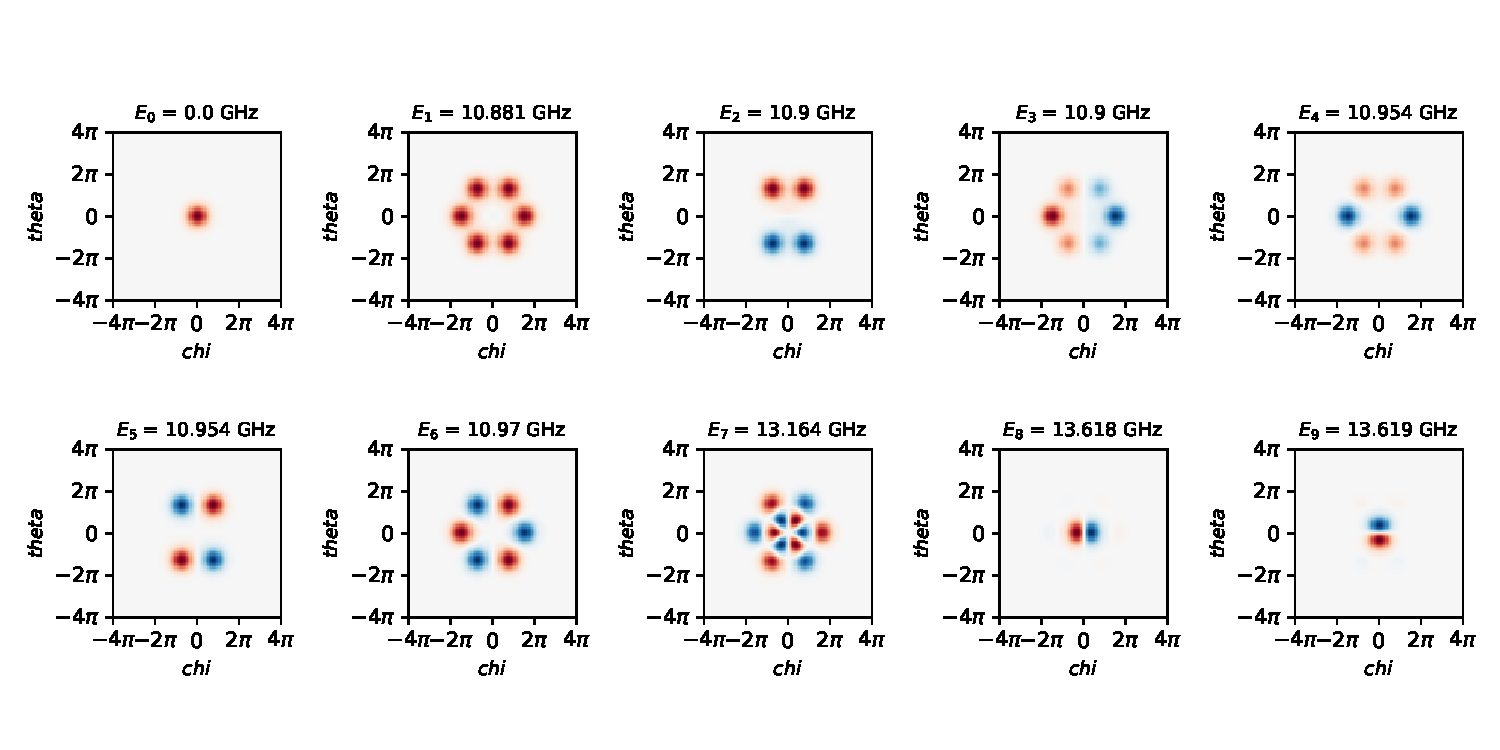
\includegraphics[trim={0cm 1.5cm 0cm 1cm}, clip, width=0.9\textwidth]{thetachi.pdf}}
	\caption{Lowest ten eigenstates of the trifluxonium with $E_C = \SI{2}{\giga\hertz}, E_J = \SI{15}{\giga\hertz}, E_L = \SI{0.3}{\giga\hertz}$. An arbitrary slice near the centre of the grid is chosen along each of the degrees of freedom $\zeta, \theta, \chi$.}
	\label{fig_estates}
\end{figure}

Three dimensional heatmaps of the eigenstates are perhaps more illuminating. We compare the ground state, which is typically designated the logical $\ket{0}$, with three excited fluxon states (Figure \ref{fig_fluxons}) and three excited plasmon states (Figure \ref{fig_plasmons}). Figure \ref{fig_fluxons} shows that the ground is indeed disjoint with the fluxons, a desirable situation between the $\ket{0}_L$ and $\ket{1}_L$ states of a qubit. Figure \ref{fig_plasmons} shows that the ground is not disjoint with the plasmons, suggesting a possibility for coupling and control.

We have chosen parameters such that the intrawell plasmons are more energetic than the disjoint interwell fluxons. This is desirable because a fluxon state can be selected as the logical $\ket{1}$, and a higher level plasmon can be used as the intermediate transition level, provided it can couple non-negligibly to both logical states. 

\begin{figure}
	\centering
	\subfigure[0th and 1st eigenstates.]{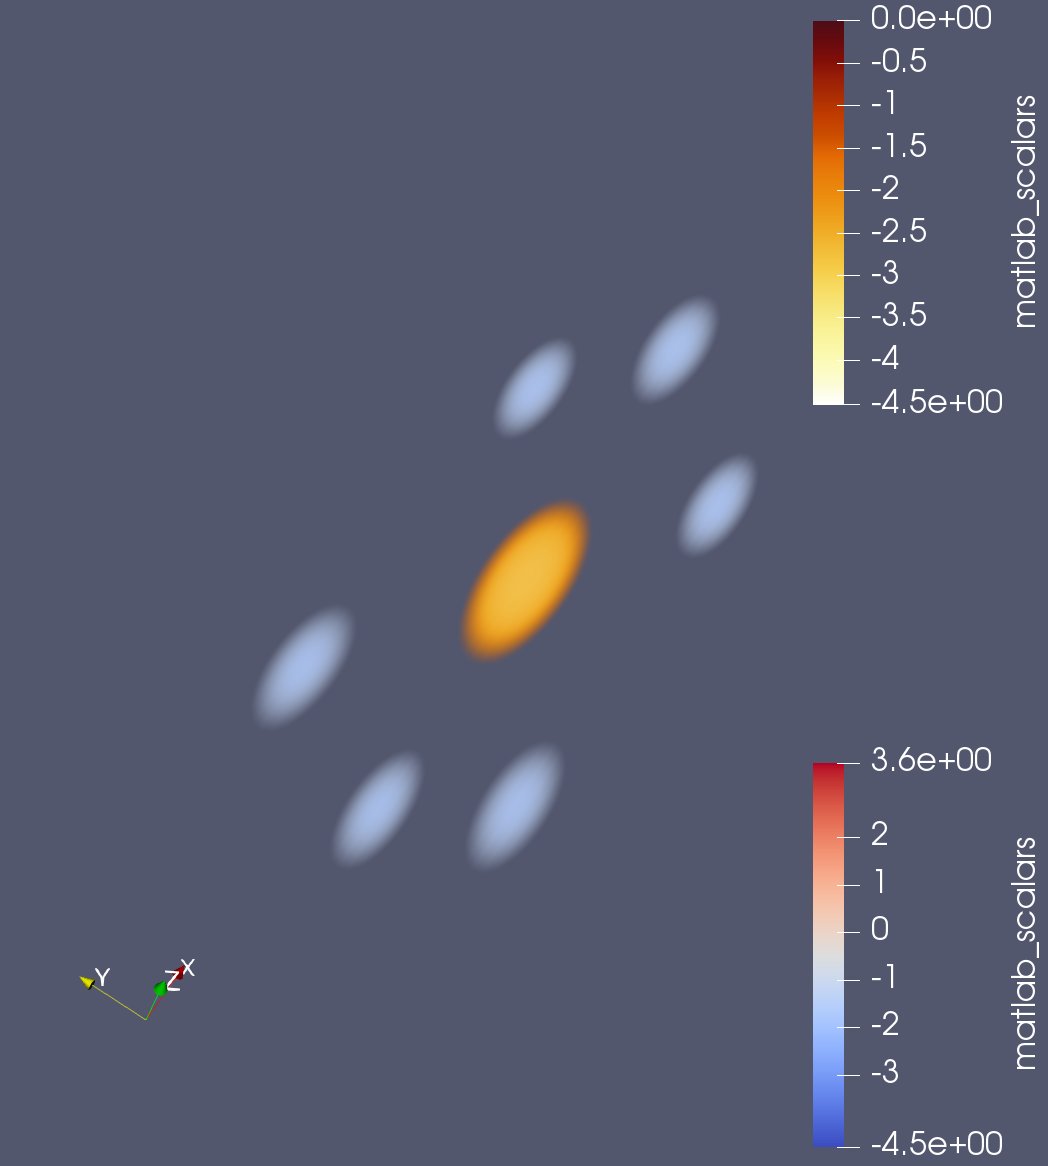
\includegraphics[width=0.25\textwidth]{ekets01.png}}
	\hspace{1em}
	\subfigure[0th and 2nd eigenstates.]{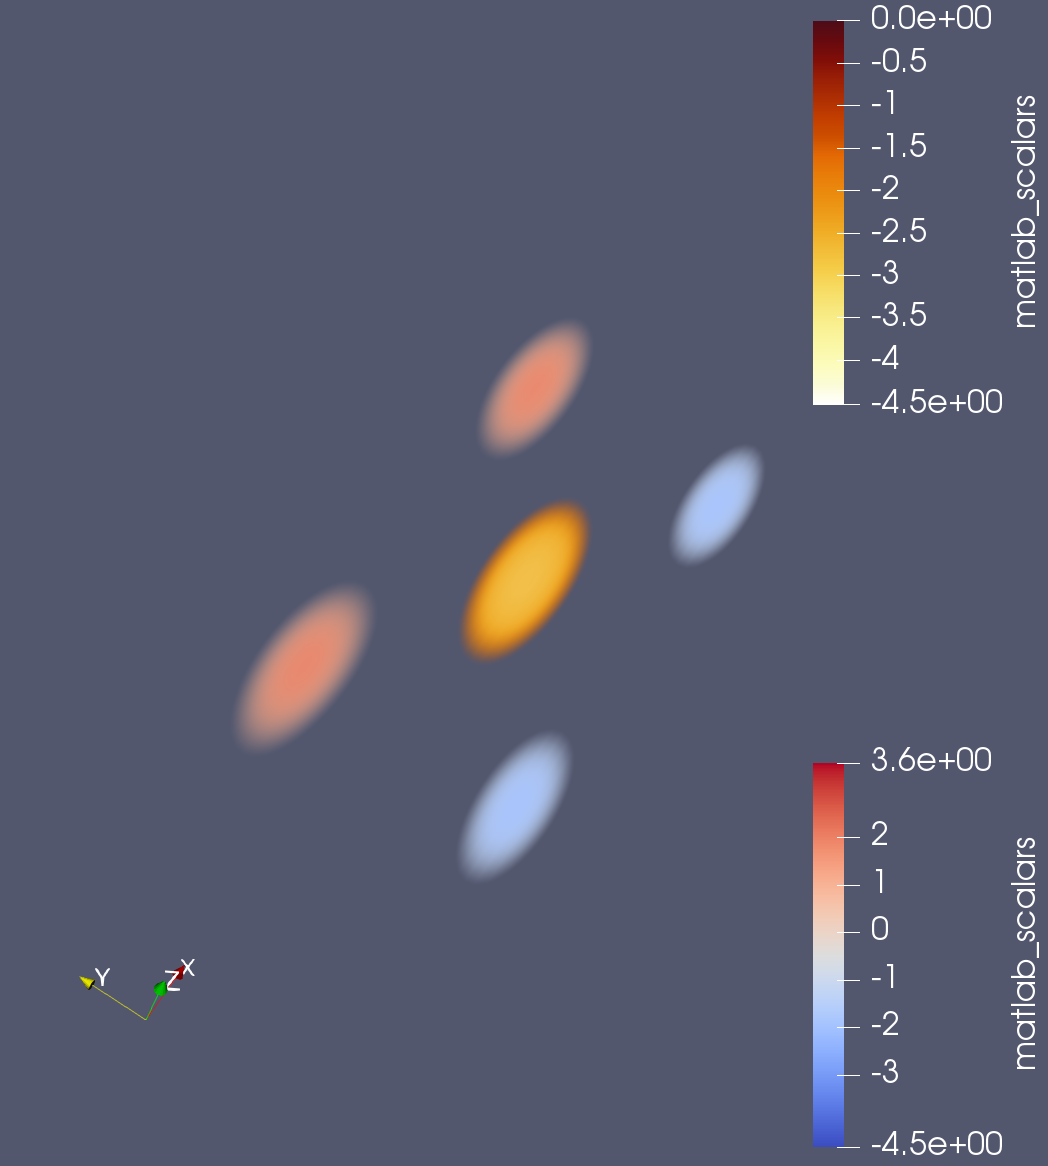
\includegraphics[width=0.25\textwidth]{ekets02.png}}
	\hspace{1em}
	\subfigure[0th and 3rd eigenstates.]{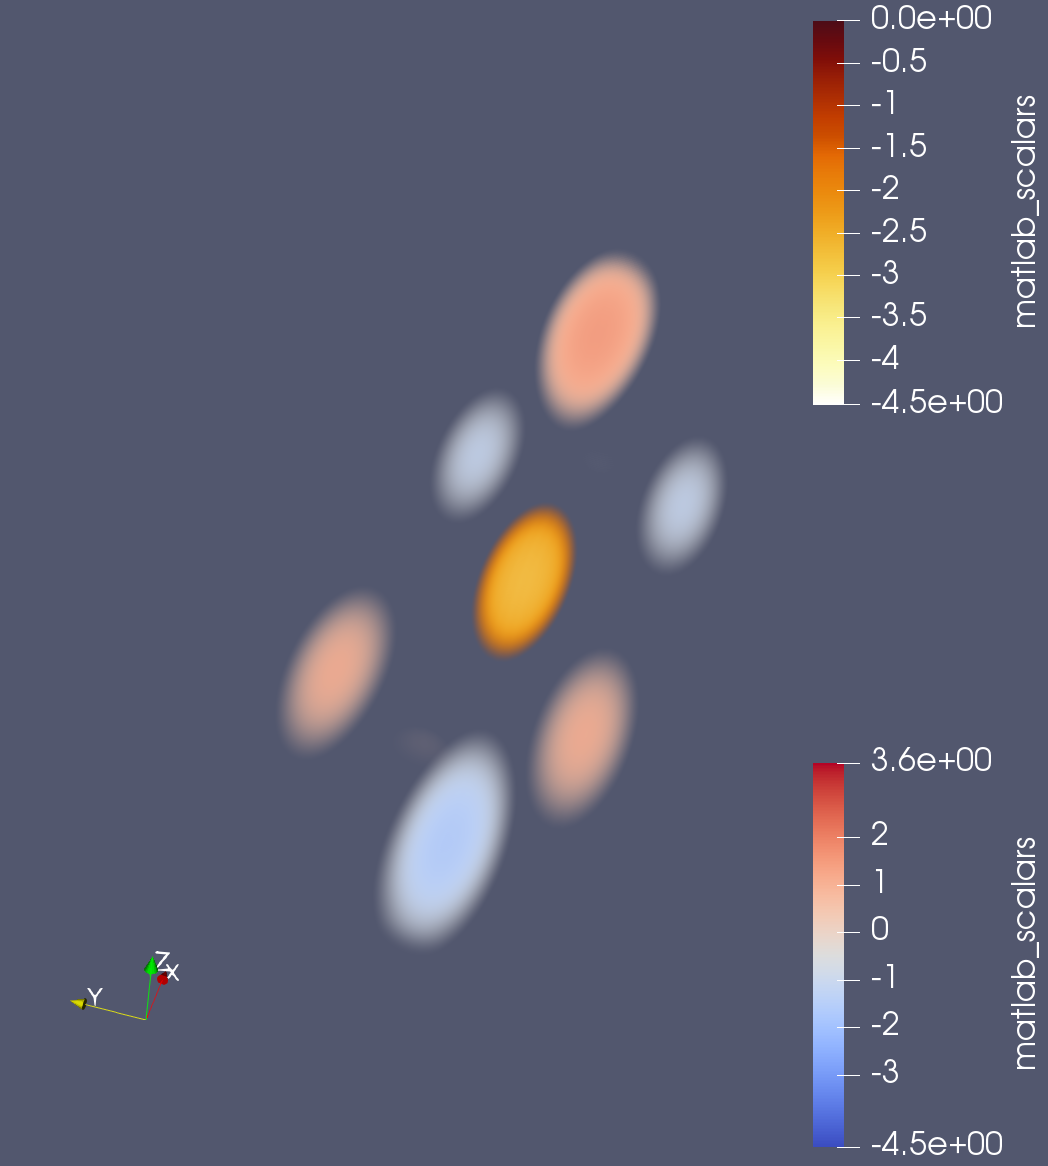
\includegraphics[width=0.25\textwidth]{ekets03.png}}
	\caption{The ground (0th) state (yellow and orange) is disjoint with the excited fluxon states (red and blue).}
	\label{fig_fluxons}
\end{figure}

\begin{figure}[H]
	\centering
	\subfigure[0th and 7th eigenstates.]{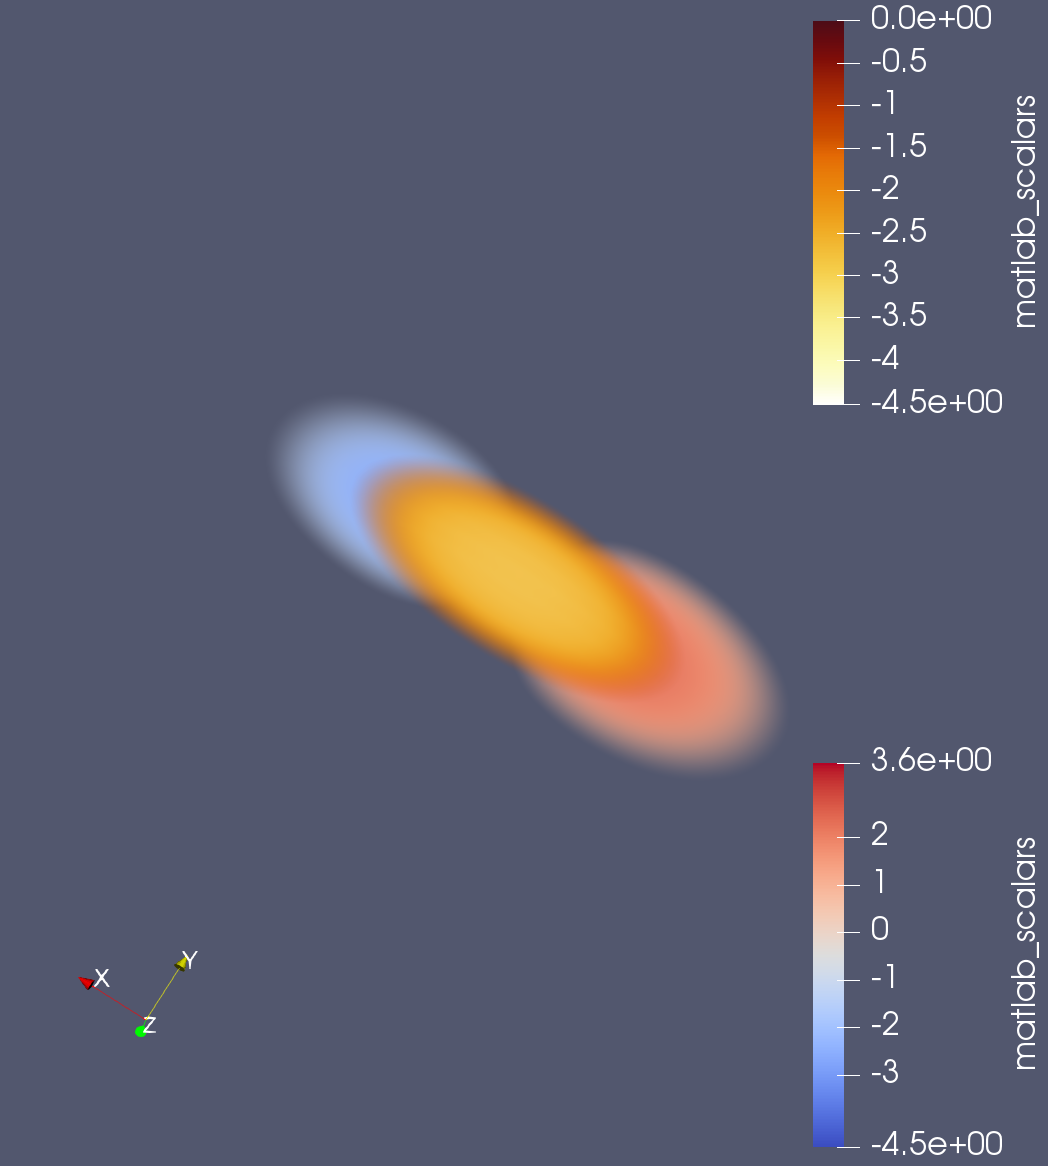
\includegraphics[width=0.25\textwidth]{ekets07.png}}
	\hspace{1em}
	\subfigure[0th and 8th eigenstates.]{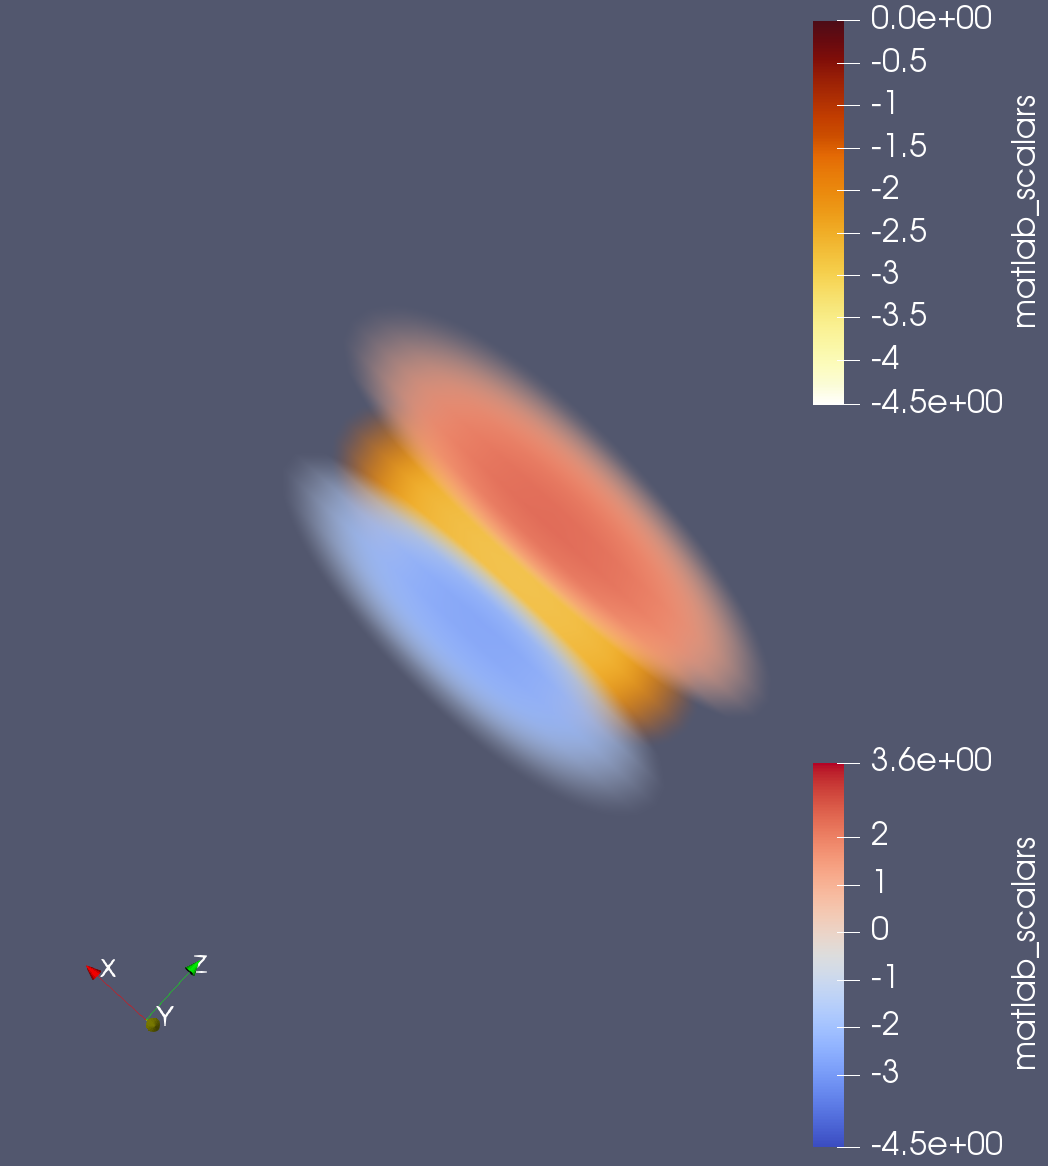
\includegraphics[width=0.25\textwidth]{ekets08.png}}
	\hspace{1em}
	\subfigure[0th and 9th eigenstates.]{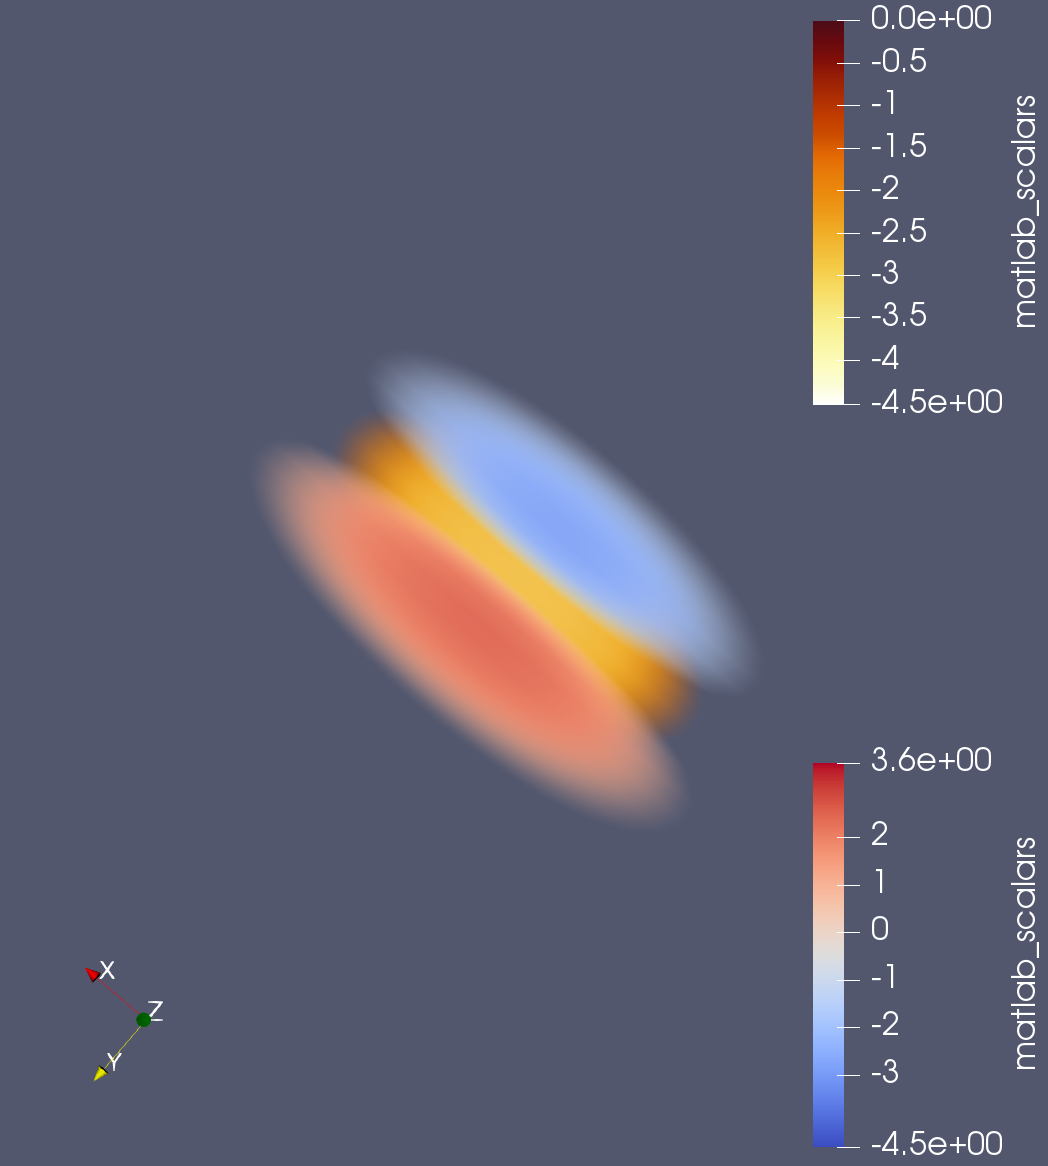
\includegraphics[width=0.25\textwidth]{ekets09.png}}
	\caption{The ground (0th) state (yellow and orange) is not disjoint with the excited plasmon states  (red and blue).}
	\label{fig_plasmons}
\end{figure}




\subsection{Capacitative coupling: $\zeta, \theta, \phi$ modes}

We derived that the trifluxonium is insensitive to external flux. Thus, let's now neglect $\phi_E$ for simplicity and work in the node rather than branch fluxes. The node phases, $\varphi_A, \varphi_B, \varphi_C, \varphi_D$ (Figure \ref{fig_trifluxcouple}) are related to original variables by
\begin{equation}
\varphi_1 = \varphi_B - \varphi_A
\hspace{1cm}
\varphi_2 = \varphi_C - \varphi_A
\hspace{1cm}
\varphi_3 = \varphi_D - \varphi_A 
\end{equation}
Different configurations of capacitative coupling, depending on the nodes coupled and the potential placed at each, achieve different coupling strengths between respective eigenstates. Generally, configurations that respect the symmetry of the phase coordinates produce the least perturbation to the Hamiltonian of the isolated qubit (does not generate other terms in the Hamiltonian in addition to the $\propto \hat{V} \otimes \hat{n}$ term). 

\begin{figure}
	\centering
	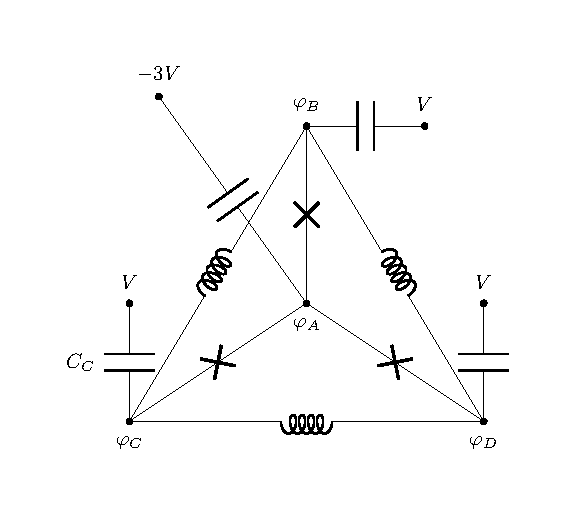
\includegraphics[trim={0cm 1cm 0cm 1cm}, clip, width=0.5\textwidth]{triflux_zeta_couple.pdf}
	\caption{$\zeta$ mode coupling of the trifluxonium. Each coupling capacitor has capacitance $C_C$ (this is independent of the capacitance of the Josephson junctions). The three outer nodes are coupled to $V$ and the centre node to $-3V$.}
	\label{fig_trifluxcouple}
\end{figure}

Figure \ref{fig_trifluxcouple} shows a configuration that follows $\zeta$ symmetries. The kinetic energy for this coupled system is
\begin{align}
T
=& \frac{1}{2} C \phi_0^2 \left((\dot{\varphi}_B - \dot{\varphi}_A)^2 + (\dot{\varphi}_C - \dot{\varphi}_A)^2 + (\dot{\varphi}_D - \dot{\varphi}_A)^2\right) + \nonumber \\
&\frac{1}{2} C_C \phi_0^2 \left((\dot{\varphi}_B - \mathcal{V})^2 + (\dot{\varphi}_C - \mathcal{V})^2 + (\dot{\varphi}_D - \mathcal{V})^2 + (\dot{\varphi}_A + 3 \mathcal{V})^2 \right) 
\end{align}
where $\mathcal{V} = \frac{V}{\phi_0}$. Diagonalisation of the kinetic energy motivates the basis
\begin{align*}
&\zeta = \frac{1}{\sqrt{12}} (-3\phi_A + \phi_B + \phi_C + \phi_D) \hspace{1cm}
\theta = \frac{1}{\sqrt{2}} (-\phi_B + \phi_C) \\
&\chi = \frac{1}{\sqrt{6}}  (-\phi_B - \phi_C + 2 \phi_D) \hspace{2cm}
\Sigma = \frac{1}{2} (\phi_A + \phi_B + \phi_C + \phi_D) \numberthis
\end{align*}
which is consistent with our original definitions of definitions of $\zeta, \theta, \chi$ in terms of $\varphi_1, \varphi_2, \varphi_3$, though we have renormalised $\zeta$ and introduced a fourth variable $\Sigma$. In these coordinates,
\begin{equation}
T = \frac{1}{2} C \phi_0^2 (4 \dot{\zeta}^2 + \dot{\theta}^2 + \dot{\chi}^2) + 
\frac{1}{2} C_C \phi_0^2 (\dot{\zeta}^2 + \dot{\theta}^2 + \dot{\Sigma}^2 - 4 \sqrt{3} \mathcal{V} \dot{\zeta} + 12 \mathcal{V}^2)
\end{equation}
where we have dropped the constant $\mathcal{V}^2$ term and $\dot{\Sigma}$, whose motion is trivial as the potential is $\Sigma$-independent. Defining $C_\zeta = 4C + C_C, C_\theta = C + C_C, C_\chi = C + C_C$, 
\begin{equation}
T = \frac{1}{2} C_\zeta \phi_0^2 \dot{\zeta}^2 + \frac{1}{2} C_\theta \phi_0^2 \dot{\theta}^2 + \frac{1}{2} C_\chi \phi_0^2 \dot{\chi}^2 + 2 \sqrt{3} C_C \phi_0 V \dot{\zeta}
\end{equation}
As no junction or inductive terms were involved in coupling, the potential (denoted $U$ to avoid confusion with the coupling potential) remains unperturbed. From $\lagr=T-U$ and $n_\varphi = \frac{1}{\hbar} \pdv{\lagr}{\dot{\varphi}}$, the conjugate charge numbers are
\begin{equation}
n_\zeta = \frac{1}{\hbar} C_\zeta \phi_0^2 \dot{\zeta} + \frac{1}{\hbar} 2 \sqrt{3} C_C \phi_0 V
\hspace{1cm}
n_\theta = \frac{1}{\hbar} C_\theta \phi_0^2 \dot{\theta}
\hspace{1cm}
n_\chi = \frac{1}{\hbar} C_\chi \phi_0^2 \dot{\chi} 
\end{equation}
Making the Legendre transform and substituting the momenta,
\begin{align}
\ham 
&= - 4 E_\zeta \left(\frac{\hbar n_\zeta - 2 \sqrt{3} C_C \phi_0 V}{C_\zeta}\right)^2 - 4 E_\theta \hbar^2 n_\theta^2  - 4 E_\chi \hbar^2 n_\chi^2 + U \\
\ham 
&= - 4 E_\zeta \partial_\zeta^2 - 4 E_\theta \partial_\theta^2  - 4 E_\chi \partial_\chi^2 + 2 \sqrt{3} (2e) \frac{C_C}{C_\zeta} V \partial_\zeta + U \\
&= \ham_0 + 2 \sqrt{3} (2e) \frac{C_C}{C_\zeta} V \partial_\zeta
\end{align}   
where $E_\zeta = \frac{e^2}{2C_\zeta}, E_\theta = \frac{e^2}{2C_\theta}, E_\chi = \frac{e^2}{2C_\chi}$. We dropped the constant $V^2$ term. This configuration couples purely the $\zeta$ degree of freedom (hence `$\zeta$ mode' coupling) and $2 \sqrt{3} (2e) \hbar \frac{C_C}{C_\zeta} V n_\zeta$ is the `$g$ coupling strength'. Thus we're interested in the numeric evaluation of the matrix dipole moments $\matrixel{i}{\partial_\zeta}{j}$ between eigenstates $\ket{i}$ and $\ket{j}$. Ideally, these moments are small between the two logical states (disjointness) but large between the intermediate transition state and each logical state.

The respective coupling terms for $\theta$ and $\chi$ mode coupling are similarly derived, by following the symmetry of each phase coordinate. The $\theta$ mode can be achieved with $-V$ at $\phi_B$, $V$ at $\phi_C$, and $0$ at $\phi_A$ and $\phi_D$, the $\chi$ mode with $-V$ at $\phi_B$ and $\phi_C$, $2V$ at $\phi_D$, and $0$ at $\phi_A$. The respective coupling strenghts are $g \propto \matrixel{i}{\partial_\theta}{j}$ and $g \propto \matrixel{i}{\partial_\chi}{j}$. 




\subsection{Capacitative coupling: numerical results}

Coupling can be treated as a perturbation on the Hamiltonian of the isolated qubit. Though it is more exact to diagonalise the coupled Hamiltonian, we can take the unperturbed eigensystem as a reasonable first order approximation to the coupled eigensystem; in particular, we will calculate the coupling matrix elements with the unperturbed eigenstates. 

Experimentally desirable $g$ coupling strengths are on the order of $\SI{e-3}{\giga\hertz}$ to $\SI{e-1}{\giga\hertz}$. We make an order of magnitude estimate for feasible matrix elements from typical values for a coupling cavity. We saw previously that for the circuit QED setup, $V \rightarrow V_\text{rms} (\hat{a} + \hat{a}^\dagger)$. Let the effective impedance of the cavity be $Z_R$. For a open $\lambda/2$ (half wave) resonator,
\begin{equation}
C_R = \frac{\pi}{2 \omega_R Z_R}
\end{equation}
So
\begin{equation}
V_\text{rms} = \sqrt{\frac{\hbar \omega_R}{2 C_R}} = \omega_R \sqrt{\frac{\hbar}{\pi} Z_R}
\end{equation}
We saw that the coupling term is on order
\begin{equation}
(2e) \frac{C_C}{C_\zeta} V_\text{rms} \frac{1}{\hbar} \matrixel{i}{\partial_\zeta}{j}
= \sqrt{\frac{4e^2}{\pi \hbar} Z_R} \frac{C_C}{C_\zeta} \omega_R \matrixel{i}{\partial_\zeta}{j}
\end{equation}
with analogous expressions for the $\theta$ and $\chi$ driving modes.

A typical resonator impedance is $Z_R \sim \SI{50}{\ohm}$, so $\sqrt{\frac{4e^2}{\pi \hbar} Z_R} \sim 0.125$. Coupling capacitances are order $C_C \sim \SI{5}{\femto\farad}$. Estimating charging energies in the circuit at $E_C \sim \SI{2}{\giga\hertz}$, we obtain that $C \sim \SI{10}{\femto\farad}$, so the ratio of capacitances is order $\SI{e-1}{}$. A typical resonator frequency is $\SI{8}{\giga\hertz}$, so $\omega_R = 2 \pi f_\text{res} \sim \SI{50}{\giga\hertz}$. Thus to achieve experimentally realistic coupling, the matrix element should be order of $\SI{e-3}{}$ to $\SI{e-1}{}$.

Figure \ref{fig_dipole} shows the coupling matrix elements. From disjointness considerations, a possible choice under $\zeta$ coupling could be $\ket{0}$ for the logical 0, $\ket{1}$ for the logical 1, and $\ket{7}$ as the intermediate transition state. Then $\ket{0}_L$ and $\ket{1}_L$ are disjoint but couple fairly strongly to the intermediate $\ket{7}$. Thus the disjoint support condition is well satisfied, and qubit control via a multistep transition should be achievable. Experimentally, the large level spacing between $\ket{0}$ and $\ket{7}$ may pose some difficulties, however.

\begin{figure}[H]
	\centering
	\subfigure{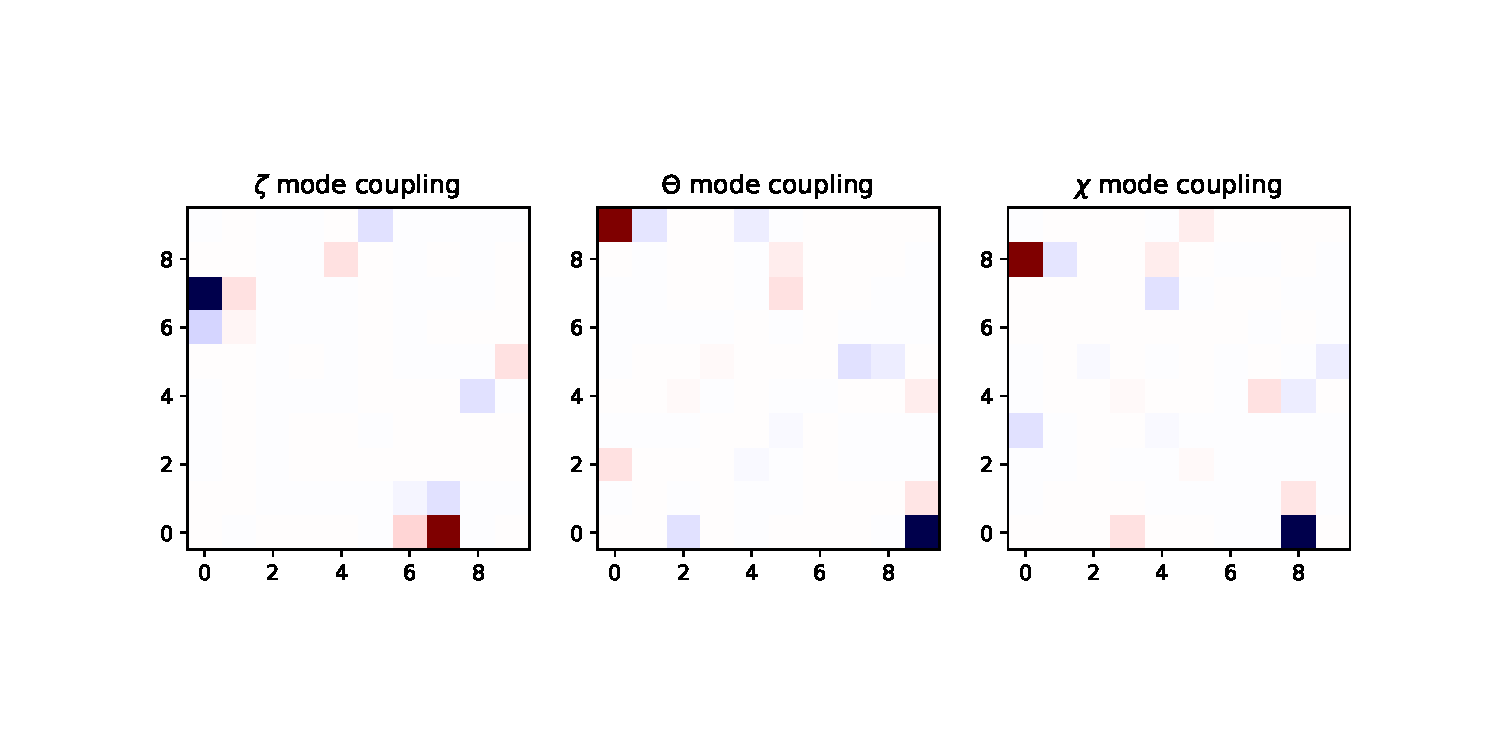
\includegraphics[trim={2cm 2.5cm 2cm 2.5cm}, clip, width=0.9\textwidth]{coupling.pdf}}
	\subfigure{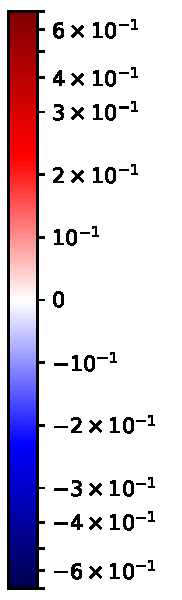
\includegraphics[trim={0cm -1cm 0cm 0cm}, clip, width=0.08\textwidth]{coupling_colorbar.pdf}}
	\caption{Matrix elements $\matrixel{i}{\partial}{j}$ for the three driving modes for the first ten eigenstates of the trifluxonium with $E_C = \SI{2}{\giga\hertz}, E_J = \SI{15}{\giga\hertz}, E_L = \SI{0.3}{\giga\hertz}$. Each cell on the symmetric grid is the matrix element between the eigenstates numbered on the axis.}
	\label{fig_dipole}
\end{figure}

\section{Conclusions}

We explored a novel superconducting qubit, the trifluxonium, by deriving analytically the system Hamiltonian and finding numerically its energy spectrum and eigenstates. It is flux-insensitive when the $\phi_\text{ext}$ is constant between the three loops, and thus quite robust to the primary source of external noise. We identified a set of parameters for which the trifluxonium achieves disjoint support between $\ket{0}$ and $\ket{1}$. An analysis of some possible capacitative coupling setups suggests a viable multistep Raman transition for controlling the qubit state. The trifluxonium's main shortcomings are its multiple degeneracies, which cannot be broken without compromising other desirable characteristics, and its large level spacings; these pose nontrivial challenges to qubit control. Nevertheless, it appears that four-node circuits do achieve some desirable qubit characteristics that their simple two-node counterparts do not, particularly with regards to disjointness. We hope this work encourages further exploration of superconducting qubits with higher degrees of freedom.



\section{Appendices}

\subsection{Finite difference method}

The finite difference method (FDM) is a discretisation technique for numerically solving differential equations. Beginning from the Taylor expansion of a function 

\begin{equation}
f(x) = \sum_{k=0}^\infty \frac{f^k(x_0)}{k!} (x-x_0)^k
\end{equation}

We usse the linear order expansion
\begin{equation}
f(x + \Delta x) = f(x) + f'(x) \Delta x + \order{\Delta x^2}
\implies f'(x) = \frac{f(x + \Delta x) - f(x)}{\Delta x} + \order{\Delta x}
\end{equation}

So to first order, we define the forward and backward differences respectively
\begin{align}
f'(x) = \frac{f(x + \Delta x) - f(x)}{\Delta x} + \order{\Delta x} \\
f'(x) = \frac{f(x) - f(x - \Delta x)}{\Delta x} + \order{\Delta x}
\end{align}

From the mean of the forward and backwards differences, we obtain the symmetric difference first derivative
\begin{equation}
f'(x) = \frac{f(x + \Delta x) - f(x - \Delta x)}{2 \Delta x} + \order{\Delta x^2}
\end{equation}

By dividing a continuous region of one-dimensional $x$-space into $n$ discretised intervals of size $\Delta x$, we obtain 
\begin{equation}
\begin{bmatrix}
	f'(x_0) \\ f'(x_1) \\ \vdots \\ f'(x_n)
\end{bmatrix}
=
\frac{1}{2 \Delta x}
\begin{bmatrix}
	0 & 1 \\
	-1 & 0 & 1 \\
	& \ddots & \ddots & \ddots \\
	& & -1 & 0 & 1 \\
	& & & -1 & 0
\end{bmatrix}
\begin{bmatrix}
	f(x_0) \\ f(x_1) \\ \vdots \\ f(x_n)
\end{bmatrix}
\end{equation}

Note that the boundaries $f'(x_0)$ and $f'(x_n)$ are somewhat off (they contain the $f(x+\Delta x)$ or $-f(x-\Delta x)$ terms only), so the boundary accuracy suffers. If the one dimensional space we're discretising has a periodic boundary condition, that is, it lies on a ring where $x_{n+1} = x_0$, the boundary conditions must be consistent with this periodicity. This is the case for compact variables periodic over $2\pi$.

\begin{equation}
f'(x_0) = \frac{f(x_1) - f(x_n)}{2 \Delta x} + \order{\Delta x^2},
\quad
f'(x_n) = \frac{f(x_0) - f(x_{n-1})}{2 \Delta x} + \order{\Delta x^2}
\end{equation}

which yields
\begin{equation}
\begin{bmatrix}
	f'(x_0) \\ f'(x_1) \\ \vdots \\ f'(x_n)
\end{bmatrix}
=
\frac{1}{2 \Delta x}
\begin{bmatrix}
	0 & 1 & & & -1 \\
	-1 & 0 & 1 \\
	& \ddots & \ddots & \ddots \\
	& & -1 & 0 & 1 \\
	1 & & & -1 & 0
\end{bmatrix}
\begin{bmatrix}
	f(x_0) \\ f(x_1) \\ \vdots \\ f(x_n)
\end{bmatrix}
\end{equation}


The same process for the second derivative yields the symmetric
\begin{equation}
f''(x) = \frac{f(x + \Delta x) - 2 f(x) + f(x - \Delta x)}{\Delta x^2} + \order{\Delta x^2}
\end{equation}

This can be represented as
\begin{equation}
\begin{bmatrix}
	f''(x_0) \\ f''(x_1) \\ \vdots \\ f''(x_n)
\end{bmatrix}
=
\frac{1}{\Delta x^2}
\begin{bmatrix}
	-2 & 1 \\
	1 & -2 & 1 \\
	& \ddots & \ddots & \ddots \\
	& & 1 & -2 & 1 \\
	& & & 1 & -2
\end{bmatrix}
\begin{bmatrix}
	f(x_0) \\ f(x_1) \\ \vdots \\ f(x_n)
\end{bmatrix}
\end{equation}

Similarly, for periodic boundary conditions where $x_{n+1} = x_0$, we have 
\begin{equation}
\begin{bmatrix}
	f''(x_0) \\ f''(x_1) \\ \vdots \\ f''(x_n)
\end{bmatrix}
=
\frac{1}{\Delta x^2}
\begin{bmatrix}
	-2 & 1 & & & 1 \\
	1 & -2 & 1 \\
	& \ddots & \ddots & \ddots \\
	& & 1 & -2 & 1 \\
	1 & & & 1 & -2
\end{bmatrix}
\begin{bmatrix}
	f(x_0) \\ f(x_1) \\ \vdots \\ f(x_n)
\end{bmatrix}
\end{equation}


In summary, the first and second derivatives (which are the only relevant derivatives for our purposes) can be expressed as operators on a discretised space. For a non-periodic space,

\begin{equation}
\dv{x} =
\frac{1}{2 \Delta x}
\begin{bmatrix}
	0 & 1 \\
	-1 & 0 & 1 \\
	& \ddots & \ddots & \ddots \\
	& & -1 & 0 & 1 \\
	& & & -1 & 0
\end{bmatrix},
\quad
\dv[2]{x} =
\frac{1}{\Delta x^2}
\begin{bmatrix}
	-2 & 1 \\
	1 & -2 & 1 \\
	& \ddots & \ddots & \ddots \\
	& & 1 & -2 & 1 \\
	& & & 1 & -2
\end{bmatrix}
\end{equation} 

For periodic boundary conditions,

\begin{equation}
\dv{x} =
\frac{1}{2 \Delta x}
\begin{bmatrix}
	0 & 1 & & & -1 \\
	-1 & 0 & 1 \\
	& \ddots & \ddots & \ddots \\
	& & -1 & 0 & 1 \\
	1 & & & -1 & 0
\end{bmatrix},
\quad
\dv[2]{x} =
\frac{1}{\Delta x^2}
\begin{bmatrix}
	-2 & 1 & & & 1 \\
	1 & -2 & 1 \\
	& \ddots & \ddots & \ddots \\
	& & 1 & -2 & 1 \\
	1 & & & 1 & -2
\end{bmatrix}
\end{equation} 

The trifluxonium Hamiltonian also contain mixed trigonometric terms (in the inductive energy). In order to apply them to separate spaces, we use sum-of-angle identities
\begin{align}
& \cos{\left(\frac{\zeta + \sqrt{2} \chi}{\sqrt{3}}\right)} + 2 \cos{\left(\frac{\theta}{\sqrt{2}}\right)} \cos{\left(\frac{\zeta}{\sqrt{3}} - \frac{\chi}{\sqrt{6}}\right)} \\
= 
& \cos{\left(\frac{\zeta}{\sqrt{3}}\right)} \cos{\left(\sqrt{\frac{2}{3}}\chi\right)} - \sin{\left(\frac{\zeta}{\sqrt{3}}\right)} \sin{\left(\sqrt{\frac{2}{3}}\chi\right)} + \\
& 2 \cos{\left(\frac{\theta}{\sqrt{2}}\right)} \cos{\left(\frac{\zeta}{\sqrt{3}}\right)} \cos{\left(\frac{\theta}{\sqrt{2}}\right)} + 2 \cos{\left(\frac{\theta}{\sqrt{2}}\right)} \sin{\left(\frac{\zeta}{\sqrt{3}}\right)} \sin{\left(\frac{\theta}{\sqrt{2}}\right)}
\end{align}


Because $\zeta, \theta, \chi$ are orthogonal directions in phase space, so we can express an arbitrary wavefunction as the outer (Kronecker) product of the operation in each of the three spaces. For example
\begin{align}
\partial_\zeta^2 &\rightarrow \partial_\zeta^2 \otimes I \otimes I \\
\theta^2 &\rightarrow I \otimes \theta^2 \otimes I \\
\cos{\zeta} \cos{\chi} &\rightarrow \cos{\zeta} \otimes I \otimes \cos{\chi}
\end{align}

The Hamiltonian can now be entirely expressed as a matrix on a region of three dimensional phase space. We decrease the increments $\Delta \zeta, \Delta \theta, \Delta \chi$ to improve simulation accuracy. Note that $\zeta$ is compact and requires the differential operators with periodic bounding conditions, while $\theta$ and $\chi$ do not. The eigenvalues of the Hamiltonian are the system's eigenergies. The eigenvectors of the Hamiltonian are the eigenstates whose value is given at each discretised grid of size $\Delta \zeta \ \Delta \theta \ \Delta \chi$.




\subsection{Trifluxonium basis transform}

The basis transform is motivated by diagonalising the linear inductance in the potential, and identifying the compact variable which lies in its nullspace (that is, the variable on which the potential purely periodically). For the trifluxonium, the inductive term is

\begin{equation}
E_\text{inductor}
= \frac{1}{2} E_L
\begin{bmatrix}
	\varphi_1 & \varphi_2 & \varphi_3
\end{bmatrix}
\begin{bmatrix}
	2 & -1 & -1 \\
	-1 & 2 & -1 \\
	-1 & -1 & 2
\end{bmatrix}
\begin{bmatrix}
	\varphi_1 \\ \varphi_2 \\ \varphi_3
\end{bmatrix}
\end{equation}

This matrix has the eigensystem: $ \frac{1}{\sqrt{3}} \begin{bmatrix} 1 & 1 & 1 \end{bmatrix}^T $ for the 0-eigenspace and $ \frac{1}{\sqrt{2}} \begin{bmatrix} -1 & 0 & 1 \end{bmatrix}^T, \frac{1}{\sqrt{6}} \begin{bmatrix} -1 & 2 & -1 \end{bmatrix}^T $ for the eigenspace with eigenvalue 3. We used Graham-Schmidt to obtain two orthonormal basis vectors in the latter eigenspace. This motivates the transformation

\begin{equation}
\begin{bmatrix}
	\varphi_1 \\
	\varphi_2 \\
	\varphi_3
\end{bmatrix}
=
\begin{bmatrix}
	\frac{1}{\sqrt{3}} & -\frac{1}{\sqrt{2}} & -\frac{1}{\sqrt{6}} \\
	\frac{1}{\sqrt{3}} & 0 					 & \frac{2}{\sqrt{6}} \\
	\frac{1}{\sqrt{3}} & \frac{1}{\sqrt{2}}  & -\frac{1}{\sqrt{6}}
\end{bmatrix}
\begin{bmatrix}
	\zeta \\ \theta \\ \chi
\end{bmatrix}
\end{equation}

which diagonalises the matrix so that the inductive term of the potential energy can be reexpressed as
\begin{equation}
E_\text{inductor}
= \frac{1}{2} E_L
\begin{bmatrix}
	\zeta & \theta & \chi
\end{bmatrix}
\begin{bmatrix}
	0 & 0 & 0 \\
	0 & 3 & 0 \\
	0 & 0 & 3
\end{bmatrix}
\begin{bmatrix}
	\zeta \\ \theta \\ \chi
\end{bmatrix}
\end{equation}
$\zeta$ is the compact variable.



\nocite{*}
\addcontentsline{toc}{section}{References}
\bibliographystyle{h-physrev}
\bibliography{draft}

% running
% pdflatex fullbib.tex
% pdflatex fullbib.tex
% then
% bibtex fullbib
% then 
% pdflatex fullbib.tex
% pdflatex fullbib.tex

\end{document}


